% !TeX program = XeLaTeX
% !TeX root = main.tex
% Edit by: 八一
\chapter{假设检验\label{cha:7}}
统计推断的另一个主要内容是统计假设检验. 在这一章里我们将讨论统计假设的设立及其检验问题.

\section{假设检验的基本思想与概念\label{sec:7.1}}
\subsection{假设检验问题\label{7.1.1}}
我们从一个例子开始引出假设检验问题.
\begin{example}\label{exam7.1.1}
某厂生产的合金强度服从正态分布 $N(\theta,16)$ ,其中 $\theta$ 的设计值为不低于 110(Pa) .为保证质量,该厂每天都要对生产情况做例行检查,以判断生产是否正常进行,即该合金的平均强度不低于 110(Pa) .某天从生产中随机抽取25块合金,测得强度值为 $x_{1},x_{2},\dotsc,x_{25}$ 其均值为 $\overline{x}=108(\mathrm {Pa})$ ,间当日生产是否正常?

对这个实际问题可作如下分析;
\begin{enumerate}
	\item 这不是一个参数估计问题.
	
	\item 这是在给定总体与样本下,要求对命题“合金平均强度不低于110 Pa”作出回答:“是”还是“否”?这类问题称为统计假设检验问题,简称假设检验问题.
	
	\item 命题:“合金平均强度不低于110 Pa”正确与否仅涉及参数0,因此该命题是否正确将涉及如下两个参数集合:
	\[
	\theta_0=\left|\theta ;\theta\geq 110\right|,\\\theta_1=\left|\theta :\theta <110\right|
	\]
	命题成立对应于 “$\theta\in\theta_0$” ,命题不成立则对应 “$\theta\in\theta_1$” .在统计学中这两个非空参数集合都称作统计假设,简称假设.
	\item 我们的任务是利用所给总体 $N(\theta,16)$ 和样本均值 $\overline{x}=108(\mathrm {Pa})$去判断假设(命题) “$\theta\in\theta_0$” .是否成立,这里的“判断”在统计学中称为检验或检验法则.
	
	检验结果有两种:
	\begin{center}
		“假设不正确”——称为拒绝该假设;
		
		“假设正确”——称为接收该假设.
	\end{center}
	\item 若假设可用一个参数的集合表示,该假设检验问题称为参数假设检验问题,否则称为非参数假设检验问题,例~\ref{exam7.1.1} 就是一个参数假设检验问题,而对假设“总体为正态分布”作出检验的问题就是一个非参数假设检验问题.本章前三节讲述参数假设检验问题,最后一节(\ref{sec:7.4})将讨论非参数假设检验问题.
\end{enumerate}

\end{example}

\subsection{假设检验的基本步骤\label{7.1.2}}
接下来我们来叙述假设检验的基本步骤.

\subsubsection{建立假设}

在假设检验中,常把一个被检验的假设称为原假设,用 $H_{0}$ 表示,通常将不应轻易加以否定的假设作为原假设.当 $H_{0}$ 被拒绝时而接收的假设称为备择假设,用 $H_{1}$ 表示,它们常常成对出现.在例~\ref{exam7.1.1} 中,我们可建立如下两个假设:
\[H _ { 0 } : \theta \in \Theta _ { 0 } = \left\{ \theta : \theta \geq 110 | \quad \text { vs } \quad H _ { 1 } ; \theta \in \Theta _ { 1 } = \{ \theta : \theta < 110 \}\right.\]
或简写为
\[H _ { 0 } : \theta \geq 110 \quad \text { vs } \quad H _ { 1 } : \theta < 110\]

其中“vs”是versus的缩写,是“对”的意思,即表示$H_{0}$对$H_{1}$的假设检验问题.

\subsubsection{选择检验统计量,给出拒绝域形式}

由样本对原假设进行判断总是通过一个统计量完成的,该统计量称为检验统计量.比如,在例~\ref{exam7.1.1}中,样本均值$\overline{x}$就是一个很好的检验统计量,因为要检验的假设是正态总体的均值,在方差已知场合,样本均值$x$是总体均值的充分统计量、使原假设被拒绝的样本观测值所在区域称为拒绝域,一般它是样本空间的一个子集,并用 $W$ 表示,在例~\ref{exam7.1.1}中,样本均值$\overline{x}$愈大,意味着总体均值 $\theta$ 也大,样本均值$\overline{x}$愈小,意味着总体均值 $\theta$ 也小,因此,在样本均值的取值中有一个临界值 $c$(待定),所以拒绝域为
\[\{W = | \left( x _ { 1 } , \cdots , x _ { n } \right) ; \overline { x } \leq c \} = \{ \overline { x } \leq c \}\]
是合理的.

当拒绝域确定了,检验的判断准则跟着也确定了:
\begin{itemize}
	\item 如果 $\left( x _ { 1 } , \cdots , x _ { n } \right) \in W$ ,则认为 $H_{0}$不成立;
	\item 如果 $\left( x _ { 1 } , \cdots , x _ { n } \right) \in \overline { W }$ ,认为 $H_{0}$成立;
\end{itemize}

一般将$\overline{W}$称为接收域.由此可见,一个拒绝域$W$唯一确定一个检验法则,反之,一个检验法则也唯一确定一个拒绝续.在两个观测值$n=2$场合,图~\ref{fig7.1.1} 给出拒绝域的示意图.

通常我们将注意力放在拒绝域上.正如在数学上我们不能用一个例子去证

明一个结论一样,用一个样本(例子)不能证明一个命题(假设)是成立的,但可以用一个例子(样本)推翻一个命题.因此,从逻辑上看,注重拒绝域是适当的.事实上,在“拒绝原假设”和“拒绝备择假设(从而接收原假设)”之间还有一个模糊域,如今我们把它并入接收域(参见图~\ref{fig7.1.1}),所以接收域是复杂的,将之称为保留域也许更恰当,但习惯上已把它称为接收域,没有必要再进行改变,只是应注意它的含义.
\begin{figure}[!ht]
  \centering
  \begin{tikzpicture}[every node/.style = {inner sep=0pt,circle,fill=white}]
  \draw [-Stealth] (-3,0)  -- (4,0) node[below]{$x_1$};
  \draw [-Stealth] (0,-2) -- (0,3.5) node [right]{$x_2$};
  \draw [thick] plot[domain=-1.5:3](\x,1.5-\x);
  \fill [pattern=north east lines](-1.5,3) -- (3,-1.5) -- (-1.5,-1.5) -- ++ (135:1.5) -- cycle;
  \draw (-1,1) node {$W$} (0,0) node[below left]{$O$} (1.5,1.5)node[rectangle]{$x_1+x_2=2c$}node[above=1em]{$\bar W$} -- (0.6,0.9) ;
\end{tikzpicture}
  \caption{拒绝域示意图\label{fig7.1.1}}
\end{figure}


\subsubsection{选择显着性水平}

检验的结果与真实情况可能吻合也可能不吻合,因此,检验是可能犯错误的.检验可能犯的错误有两类:其一是 $H_{0}$ 为真但由子随机性使样本观测值落在拒绝域中,从而拒绝原假设$H_{0}$,这种错误称为第一类错误,其发生的概率称为犯第一类错误的概率,或称拒真概率,通常记为$\alpha$,即
\begin{equation}\label{eq7.1.1}
\alpha =P\left(\text{拒绝}H_0\left| H_0\text{为真}\right.\right)=P\left(X\in W\right),\theta\in\theta_0
\end{equation}
其中$X= \left( x _ { 1 } , \dotsc , x _ { n } \right)$表示样本.另一种错误是$H_{0}$不真(即$H_{1}$为真)但由于随机性使样本观测值落在接受域中,从而接受原假设$H_{0}$,这种错误称为第二类错误,其发生的概率称为犯第二类错误的概率,或称受伪概率,通常记为$\beta$,即
\begin{equation}\label{eq7.1.2}
\alpha =P\left(\textrm{接受}H_0\left| H_0\textrm{为真}\right.\right)=P\left(X\in \overline{ W }\right),\theta\in\Theta_0
\end{equation}

表\ref{table7.1.1}列出了检验的各种情况及两类错误.
\begin{table}[!htp]
	\centering
	\caption{检验的两类错误}\label{table7.1.1}
		\begin{tabular}{lll}
	\hline
\multirow{2}{*}{观察数据情况} & \multicolumn{2}{l}{\hspace{4em}总体情况} \\ \cline{2-3}
& $H_{0}$为真   & $H_{1}$为真     \\ \hline
$(x_{1},\dotsc,x_{n})\in W$ & 犯第一类错误 & 正确  \\
$(x_{1},\dotsc,x_{n})\in W^{c}$   & 正确  & 犯第二类错误        \\ \hline
	\end{tabular}
\end{table}

犯第一类错误的概率 $\alpha$ 和犯第二类错误的概率 $\beta$ 可以用同一个函数表示,即所谓的势函数.势函数是假设检验中最重要的概念之一,它的定义如下:
\begin{definition}{}{ybjz}
	设检验问题
	\[H _ { 0 } : \theta \in \Theta _ { 0 } \quad \text { vs } \quad H _ { 1 } : \theta \in \Theta  _ { 1 }\]
	的拒绝域为$W$,则样本观测值$X$落在拒绝域$W$内的概率称为该检验的\textbf{势函数},\index{S!势函数}记为
	\begin{equation}\label{eq7.1.3}
	g\left(\theta\right)=P_{\theta}\left(X\in  W\right),\quad\theta\in\boldsymbol{\Theta }=\Theta_0\cup\Theta_1
	\end{equation}
\end{definition}
显然,势函数 $g(\theta)$ 是定义在参数空间$\Theta$上的一个函数.由 \eqref{eq7.1.1} 和 \eqref{eq7.1.2} 知,当$\theta \in \Theta_{ 0 }$时,$g ( \theta ) = \alpha = \alpha ( \theta )$,当$\theta \in \Theta_{1 }$时,$g ( \beta ) = 1-\beta = 1-\beta ( \theta )$.由此可见,犯两类错误的概率都是参数$\theta$的函数,并可由势函数得到,即:
\[
g\left(\theta\right)=\left\{\begin{matrix}
\alpha\left(\theta\right),&		\theta\in\Theta_0\\
1-\beta\left(\theta\right),&		\theta\in\Theta_1\\
\end{matrix}\right.
\]
对例~\ref{exam7.1.1},其拒绝域为$W = | \overline{ x } \leq c |$,由(\ref{eq7.1.3})可以算出该检验的势函数
\[
g\left(\theta\right)=P_{\theta}\left(\overline{x}\leq c\right)=P_{\theta}\left(\frac{\overline{x}-\theta}{4/5}\le\frac{c-\theta}{4/5}\right)=\Phi\left(\frac{c-\theta}{4/5}\right)
\]
这个势函数是$\theta$的减函数(见图\ref{fig7.1.2})
\begin{figure}[htbp]
	\centering
	\begin{tikzpicture}
  \draw [Stealth-Stealth] (0,4) node [right]{$g$}
    -- (0,0) node(O)[below left]{$O$} -- (8,0) node [right]{$\theta$};
    \draw [thick] (0,2.8) [bend left=10] to (3.5,0.9) coordinate(a) [bend right=5] to (3.7,0.8)[bend right =10]to(7.1,0.05);
    \draw [densely dashed,thick](0,0.9) node [left]{$\alpha$} -- (a) -- (3.5,0)coordinate(b)
    (0,3.2)node[left]{1} -- (3.7,3.2) ;
    \draw (2.3,2.7) node[above=-2pt]{$g(\theta)$} -- ++ (-140:0.85);
    \draw[decorate,decoration = {brace,amplitude=0.6em}](3.5,-0.1) --node[below=3pt]{\hskip3pt$\Theta_1$} (0,-0.1);
    \draw[decorate,decoration = {brace,amplitude=0.6em}](8,-0.1) --node[below=3pt]{\hskip3pt$\Theta_0$} (3.5,-0.1);
\end{tikzpicture}
	\caption{例 \ref{exam7.1.1} 的势函数$g(\theta)$}\label{fig7.1.2}
\end{figure}

利用这个势函数容易写出其犯两类错误的概率分别为
\begin{equation}\label{eq7.1.4}
\alpha\left(\theta\right)=\Phi\left(\frac{c-\theta}{4/5}\right),\quad\theta\in\Theta_0
\end{equation}
\begin{equation}\label{eq7.1.5}
\beta\left(\theta\right)=1-\Phi\left(\frac{c-\theta}{4/5}\right),\quad\theta\in\Theta_1
\end{equation}
由上述两个式子可以看出犯两类错误的概率$\alpha,\beta$间的关系:
\begin{itemize}
	\item 当$\alpha$减小时,由 \eqref{eq7.1.4} 知,$c$也随之减小,再由 \eqref{eq7.1.5} 知,$c$的减小必导致$\beta$的增大;
	\item 当$\beta$减小时,由 \eqref{eq7.1.5} 知,$c$会增大,再由 \eqref{eq7.1.4} 知,$c$的增大必导致$\alpha$的增大.
	
\end{itemize}

这一现象说明:在样本量给定的条件下,$\alpha$与$\beta$中一个减小必导致另一个增大,这不是偶然的,而具有一般性.这进一步说明:在样本量一定的条件下不可能找到一个使$\alpha,\beta$都小的检验.在此背景下,只能采取折中方案.英国统计学家Neyman和Pearson 提出水平为$\alpha$的显著性检验的概念.
\begin{definition}{}{ybjz}
	对检验问题$H _ { 0 } : \theta \in \Theta _ { 0 } \quad \text { vs } \quad H _ { 1 } : \theta \in \Theta _ { 1 }$,如果一个检验满足对任意的$\theta \in \Theta _ { 0 }$,都有
	\[g ( \theta ) \leq \alpha\]
	则称该检验是\textbf{显着性水平}\index{J!假设检验!显著性水平}为$\alpha$的\textbf{显着性检验},\index{J!假设检验!显著性检验}简称水平为$\alpha$的检验.
\end{definition}
提出显著性检验的概念就是要控制犯第一类错误的概率$\alpha$,但也不能使得$\alpha$过小($\alpha$过小会导致$\beta$过大),在适当控制$\alpha$中制约$\beta$.最常用的选择是$\alpha=0.05$,有时也选择$\alpha=0.10$或$\alpha=0.01$.

\subsubsection{给出拒绝域}

在确定显著性水平后,我们可以定出检验的拒绝域$W$. 在例~\ref{exam7.1.1}中,若取$\alpha=0.05$,则要求对任意的$\theta\geq 100$有$g ( \theta ) = \Phi ( 5 ( c - \theta ) / 4 ) \leq 0.05$,由于$g(\theta)$是关于$\theta$的单调减函数(见图~\ref{fig7.1.2}),只需要
\[g ( 110 ) = \Phi ( 5 ( c - 110 ) / 4 ) = 0.05\]
成立即可.由此可先确定标准正态分布的0.05分位数$u _ { 0.05 } = - u _ { 0.95 }$,它使得
\[\frac { 5 ( c - 110 ) } { 4 } = u _ { 0.05 }\]
从而$c$的值为
\[c = 110 + 0.8 u _ { 0.05 } = 110 - 0.8 \times 1.645 = 108.684\]
所以,检验的拒绝域为
\[W = \{\overline { x } \leq 108.684 \}\]
若令$u = \frac { \overline { x } - 110 } { 4 / 5 }$,则拒绝域有另一种表示,即
\[W = \left\{ u \leq u _ { 0.05 } \right\} = \{ u \leq - 1.645 \}\]

\subsubsection{做出判断}

在有了明确的拒绝域$W$后,根据样本观测值我们可以做出判断:
\begin{itemize}
	\item 当$\overline{x}\leq 108.684$或$u\leq -1.645$时,则拒绝$H_{0}$,即接收$H_{1}$;
	\item 当$\overline{ x }>108.684$或$u> -1.645$时,则接收$H_{0}$.
\end{itemize}

在例~\ref{exam7.1.1} 中,由于
\[\overline { x } = 108 < 108.684\]
因此拒绝原假设,即认为该日生产不正常.
\begin{xiti}
	\item 设$x_1,\dotsc ,x_n$是来自 $N(\mu ,1)$ 的样本,考虑如下假设检验问题
	\[H _ { 0 } : \mu = 2 \quad \text { vs } \quad H _ { 1 } , \mu = 3\]
	若检验由拒绝域为 $w = \{ \overline { x } \geq 2.6 \}$ 确定.
	\begin{enumerate}
		\item 当 $n=20$ 时求检验犯两类错误的概率;
		\item 如果要使得检验犯第二类错误的概率$\beta \leq 0.01$,$n$最小应取多少?
		
		\item 证明:当 $n\rightarrow +\infty $时,$\alpha \rightarrow  0$,$\beta \rightarrow  0$.
	\end{enumerate}
	\item 设$x_1,\dotsc ,x_{10}$是来自 $0-1$ 总体 $b(1,p)$ 的样本,考虑如下检验问题
	\[H _ { 0 } : p = 0.2 \quad \text { vs } \quad H _ { 1 } , p = 0.4\]
	取拒绝域为$W = \{ \overline { x } \geq 0.5 \}$,求该检验犯两类错误的概率.
	
	\item 设$x _ { 1 } , \dotsc , x _ { 16 }$是来自正态总体$N(\mu,4)$的样本,考虑检验问题
	\[H _ { 0 } : \mu = 6 \quad \text { vs } \quad H _ { 1 } : \mu \neq 6\]
	拒绝域取为$W=\left\{\left|\overline{x}-6\right|\geq c\right\}$,试求$c$使得检验的显著性水平为0.05,并求该检验在$\mu =6.5$ 处犯第二类错误的概率.
	
	\item 设总体为均匀分布$U ( 0 , \theta ) , x _ { 1 } , \dotsc , x _ { n }$是样本,考虑检验问题
	\[H _ { 0 } : \theta \geq 3 \quad \text { vs } \quad H _ { 1 } : \theta < 3\]
	拒绝域取为$W = \{ x _ { ( n ) } \leq 2.5 \}$,求检验犯第一类错误的最大值$\alpha$,若要使得该最大值$\alpha$不超过0.05,$n$至少应取多大?
	
	\item 在假设检验问题中,若检验结果是接受原假设,则检验可能犯哪一类错误?若检验结构是拒绝原假设,则又有可能犯哪一类错误?
		
\end{xiti}


\section{正态总体参数假设检验\label{sec:7.2}}
参数假设检验常见的有三种基本形式

\[\begin{array} { l } { \text { (1) } H _ { 0 } : \theta \leq \theta _ { 0 } \quad \text { vs } H _ { 1 } : \theta > \theta _ { 0 } } \\ { \text { (2) } H _ { 0 } : \theta \geq \theta _ { 0 } \quad \text { vs } H _ { 1 } ; \theta < \theta _ { 0 } } \\ { \text { (3) } H _ { 0 } : \theta = \theta _ { 0 } \quad \text { vs } H _ { 1 } : \theta \neq \theta _ { 0 } } \end{array}\]

一般说来,对这三种假设所采用的检验统计量是相同的,差别在拒绝域上.当备择假设 $H_{1}$ 在原假设 $H_{0}$ 一侧时的检验称为\textbf{单侧检验}\index{Y!单侧检验},当备择假设 $H_{1}$ 分散在原假设 $H_{0}$ 两侧时的检验称为\textbf{双侧检验}\index{Y!双侧检验}.以上(1),(2)是单侧检验,(3)是双侧检验.识别单侧与双侧检验有益于以后构造其拒绝域.

本节对正态总体参数检验分别进行讨论.
\subsection{单个正态总体均值的检验\label{7.2.1}}
设$x _ { 1 } , \dotsc , x _ { n }$是来自$N(\mu ,\sigma^{2})$的样本,考虑如下三种关于$\mu $的检验问题
\begin{equation}\label{eq7.2.1}
H _ { 0 } : \mu \leq \mu _ { 0 } \quad \text { vs } \quad H _ { 1 } : \mu > \mu _ { 0 }
\end{equation}
\begin{equation}\label{eq7.2.2}
H _ { 0 } : \mu \geq \mu _ { 0 } \quad \text { vs } \quad H _ { 1 } : \mu < \mu _ { 0 }
\end{equation}
\begin{equation}\label{eq7.2.3}
H _ { 0 } : \mu = \mu _ { 0 } \quad \text { vs } \quad H _ { 1 } : \mu \neq \mu _ { 0 }
\end{equation}
由于正态总体含两个参数,总体方差$\sigma^{2}$已知与否对检验有影响.下面我们分$\sigma$已知和未知两种情况叙述.

\subsubsection{$\sigma$已知时的$\mu$检验}

对于单侧检验问题(\ref{eq7.2.1}),由于$\mu $的点估计是,且$\overline { x } \sim N \left( \mu , \sigma ^ { 2 } / n \right)$,故选用检验统计量
\begin{equation}\label{eq7.2.4}
u = \frac { \overline { x } - \mu _ { 0 } } { \sigma / \sqrt { n } }
\end{equation}
是恰当的.直觉告诉我们:当样本均值$\overline{x}$不超过设定均值$\mu_{ 0 }$时,应接收原假设;当样本均值$\overline{x}$超过$\mu_{ 0 }$时,应拒绝原假设.可是,在有随机性存在的场合,如果$\overline{x}$比$\mu_{ 0 }$大一点就拒绝原假设似乎不当,只有当$\overline{x}$比$\mu_{ 0 }$大到一定程度时拒绝原假设才是恰当的,这就存在一个临界值$c$,拒绝域为
\begin{equation}\label{eq7.2.5}
W = \left\{ \left( x _ { 1 } , \cdots , x _ { n } \right) : u \geq c \right\}
\end{equation}
常简记为${\mu \geq c}$,若要求检验的显著性水平为$\alpha$,则$c$满足
\[P _ { \mu _ { 0 } } ( u \geq c ) = \alpha\]
由于在$\mu =\mu_{0}$时$\mu \sim N(0,1)$,故$c=\mu _{1-\alpha}$(见图~\ref{fig7.2.1}(a)),最后的拒绝域为
\begin{equation}\label{eq7.2.6}
W = \left\lbrace  u \geq u _ { 1 - \alpha }\right\rbrace
\end{equation}
\begin{figure}[htbp]
	\centering
    \subfloat[$H_1:\mu>\mu_0$]{
      \begin{tikzpicture}[thick,yscale = 9,xscale=0.5]
  \draw (-4,0) -- (4,0) -- (4,0.4) -- (-4,0.4) -- cycle;
  \foreach \x in {-4,...,4}
    {
      \draw (\x,0) node [below]{$\x$} -- ++(0,0.01);
      \draw (\x,0.4) -- ++(0,-0.01);
    }
  \foreach \y in {0,0.1,0.2,0.3,0.4}
    \draw (-4,\y) node[left]{$\y$} -- ++ (0.1,0)
     (4,\y) node[right]{$\y$} -- ++ (-0.1,0);
  \foreach \y in {0.05,0.15,0.25,0.35}
    \draw (-4,\y) node [left]{$\y$} -- ++(0.1,0)
    (4,\y) node [right]{$\y$} -- ++(-0.1,0);
  \draw[samples=100,very thick] plot[domain=-4:4] (\x,{0.4*e^(-(\x)^2/2.5)});
  \fill[pattern = north east lines] (4,0) -- plot[domain=4:1.8](\x,{0.4*e^(-(\x)^2/2.5)}) -- (1.8,0);
  \draw (1.8,0)node[below=0.35cm]{$u_{1-\alpha}$} -- (1.8,{0.4*e^(-1.8^2/2.5)});
\end{tikzpicture}
    }\;
    \subfloat[$H_1:\mu<\mu_0$]{
      \begin{tikzpicture}[thick,yscale = 9,xscale=0.5]
  \draw (-4,0) -- (4,0) -- (4,0.4) -- (-4,0.4) -- cycle;
  \foreach \x in {-4,...,4}
    {
      \draw (\x,0) node [below]{$\x$} -- ++(0,0.01);
      \draw (\x,0.4) -- ++(0,-0.01);
    }
  \foreach \y in {0,0.1,0.2,0.3,0.4}
    \draw (-4,\y) node[left]{$\y$} -- ++ (0.1,0)
     (4,\y) node[right]{$\y$} -- ++ (-0.1,0);
  \foreach \y in {0.05,0.15,0.25,0.35}
    \draw (-4,\y) node [left]{$\y$} -- ++(0.1,0)
    (4,\y) node [right]{$\y$} -- ++(-0.1,0);
  \draw[samples=100,very thick] plot[domain=-4:4] (\x,{0.4*e^(-(\x)^2/2.5)});
  \fill[pattern = north east lines] (-4,0) -- plot[domain=-4:-1.8](\x,{0.4*e^(-(\x)^2/2.5)}) -- (-1.8,0);
  \draw (-1.8,0)node[below=0.35cm]{$u_\alpha$} -- (-1.8,{0.4*e^(-1.8^2/2.5)});
\end{tikzpicture}
    }
  \subfloat[$H_1:\mu\ne\mu_0$]{
    \begin{tikzpicture}[thick,yscale = 9,xscale=0.5]
  \draw (-4,0) -- (4,0) -- (4,0.4) -- (-4,0.4) -- cycle;
  \foreach \x in {-4,...,4}
    {
      \draw (\x,0) node [below]{$\x$} -- ++(0,0.01);
      \draw (\x,0.4) -- ++(0,-0.01);
    }
  \foreach \y in {0,0.1,0.2,0.3,0.4}
    \draw (-4,\y) node[left]{$\y$} -- ++ (0.1,0)
     (4,\y) node[right]{$\y$} -- ++ (-0.1,0);
  \foreach \y in {0.05,0.15,0.25,0.35}
    \draw (-4,\y) node [left]{$\y$} -- ++(0.1,0)
    (4,\y) node [right]{$\y$} -- ++(-0.1,0);
  \draw[samples=100,very thick] plot[domain=-4:4] (\x,{0.4*e^(-(\x)^2/2.5)});
  \fill[pattern = north east lines] (4,0) -- plot[domain=4:1.8](\x,{0.4*e^(-(\x)^2/2.5)}) -- (1.8,0);
  \draw (-1.8,0)node[below=0.35cm]{$u-_{1-\alpha/2}$} (1.8,0)node[below=0.35cm]{$u_{1-\alpha/2}$} -- (1.8,{0.4*e^(-1.8^2/2.5)});
\end{tikzpicture}
  }
	\caption{$\mu $检验的拒绝域}\label{fig7.2.1}
\end{figure}

该检验用的检验统计量是$\mu $统计量,故一般称为$\mu $检验.该检验的势函数是$\mu $的函数,它可用正态分布写出,具体如下:对$\mu \in(\infty,+\infty)$,
\begin{align*}
g ( \mu ) &= P _ { \mu } ( X \in W ) = P _ { \mu } \left( u \geq u _ { 1 - \alpha } \right)\\
&= P _ { \mu } \left( \frac { \overline { x } - \mu _ { 0 } } { \sigma / \sqrt { n } } \geq u _ { 1 - a } \right)\\
&= P _ { \mu } \left( \frac { \overline { x } - \mu + \mu - \mu _ { 0 } } { \sigma / \sqrt { n } } \geq u _ { 1 - \alpha } \right)\\
&= P _ { \mu } \left( \frac { \overline { x } - \mu } { \sigma / \sqrt { n } } \geq \frac { \mu _ { 0 } - \mu } { \sigma / \sqrt { n } } + u _ { 1 - \alpha } \right)\\
&= 1 - \Phi \left( \sqrt { n } \left( \mu _ { 0 } - \mu \right) / \sigma + u _ { 1 - a } \right)
\end{align*}
由此可见,势函数是$\mu $的增函数,其图形见图~\ref{fig7.2.2}(a),由增函数性质知,只要$g(\mu_{0}=\alpha)$就可保证在$\mu \leq \mu_{ 0 }$时有$g(\mu )\leq \mu_{ 0 }$,所以上述求出的检验是水平为$\alpha$的检验.
\begin{figure}[htbp]
	\centering
	\subfloat[$H_1:\mu>\mu_0$]{
      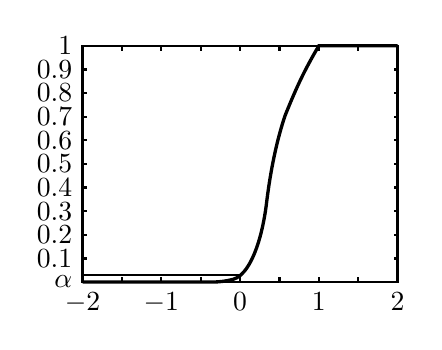
\begin{tikzpicture}[thick,yscale=3]
  \draw (-2,0) -- (2,0) -- (2,1) -- (-2,1) -- cycle;
  \foreach \x in {-2,...,2}
    \draw (\x,0)node[below]{$\x$} -- ++(0,0.02)
    (\x,1) --++ (0,-0.02);
  \foreach \x in {-1.5,-0.5,0.5,1.5}
    \draw (\x,0) -- ++(0,0.02)
    (\x,1) --++ (0,-0.02);
  \foreach \y in {0.1,0.2,0.3,0.4,0.5,0.6,0.7,0.8,0.9,1}
    \draw (-2,\y)node[left]{$\y$} -- ++(0.05,0)
    (2,\y) -- ++(-0.05,0);
  \draw (-2,0) node[left]{$\alpha$};
  \draw (0,0) -- (0,0.03) -- (-2,0.03) -- (-2,0) --cycle;
  \draw [very thick] (-2,0) -- (-0.35,0) arc(-90:-85:3)arc(-85:-40:0.5)
  arc(-40:-20:0.5)arc(160:135:1)
  [bend left=5] to (1,1) -- (2,1);
\end{tikzpicture}
    }\;
    \subfloat[$H_1:\mu<\mu_0$]{
      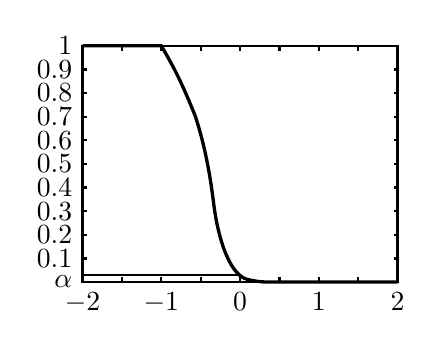
\begin{tikzpicture}[thick,yscale=3]
  \draw (-2,0) -- (2,0) -- (2,1) -- (-2,1) -- cycle;
  \foreach \x in {-2,...,2}
    \draw (\x,0)node[below]{$\x$} -- ++(0,0.02)
    (\x,1) --++ (0,-0.02);
  \foreach \x in {-1.5,-0.5,0.5,1.5}
    \draw (\x,0) -- ++(0,0.02)
    (\x,1) --++ (0,-0.02);
  \foreach \y in {0.1,0.2,0.3,0.4,0.5,0.6,0.7,0.8,0.9,1}
    \draw (-2,\y)node[left]{$\y$} -- ++(0.05,0)
    (2,\y) -- ++(-0.05,0);
  \draw (-2,0) node[left]{$\alpha$};
  \draw (0,0) -- (0,0.03) -- (-2,0.03) -- (-2,0) --cycle;
  \draw [very thick,xscale=-1] (-2,0) -- (-0.35,0) arc(-90:-85:3)arc(-85:-40:0.5)
  arc(-40:-20:0.5)arc(160:135:1)
  [bend left=5] to (1,1) -- (2,1);
\end{tikzpicture}
    }
    \subfloat[$H_1:\mu\ne\mu_0$]{
     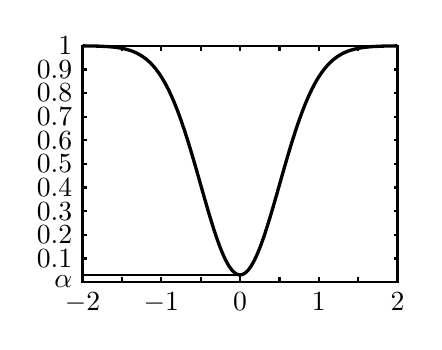
\begin{tikzpicture}[thick,yscale=3]
  \draw (-2,0) -- (2,0) -- (2,1) -- (-2,1) -- cycle;
  \foreach \x in {-2,...,2}
    \draw (\x,0)node[below]{$\x$} -- ++(0,0.02)
    (\x,1) --++ (0,-0.02);
  \foreach \x in {-1.5,-0.5,0.5,1.5}
    \draw (\x,0) -- ++(0,0.02)
    (\x,1) --++ (0,-0.02);
  \foreach \y in {0.1,0.2,0.3,0.4,0.5,0.6,0.7,0.8,0.9,1}
    \draw (-2,\y)node[left]{$\y$} -- ++(0.05,0)
    (2,\y) -- ++(-0.05,0);
  \draw (-2,0) node[left]{$\alpha$};
  \draw (0,0) -- (0,0.03) -- (-2,0.03) -- (-2,0) --cycle;
  \draw [very thick,samples=100] plot [domain=-2:2] (\x,{1-0.97*e^(-2*(\x)^2)});
\end{tikzpicture}
    }
	\caption{$g(\mu ) $的图形}\label{fig7.2.2}
\end{figure}

对单侧检验问题($\ref{eq7.2.1}$),可以类似进行讨论.仍选用$\mu $作为检验统计量,考虑到($\ref{eq7.2.1}$)的备择假设$H_{1}$在左侧,故其拒绝城应有如下形式
\[
W=\left\{\mu\le c\right\}
\]
对给定的显著性水平$\alpha(0<\alpha<1)$,由$P _ { \mu _ { 0 } } ( u \leq c ) = \alpha$可定出$c=\mu_{\alpha}$(图~\ref{fig7.2.1}(b)),最后的拒绝域为
\begin{equation}\label{eq7.2.7}
W=\left\{\mu\le\mu_{\alpha}\right\}
\end{equation}

判断准则是类似的:当$\mu\le\mu_{\alpha}$时拒绝原假设$H_{0}$(接收$H_{1}$),否则接收$H_{0}$.该检验的势函数也是$\mu $的减函数(图~\ref{fig7.2.2}(b)),具体如下:对$\mu \in(-\infty,+\infty)$,
\begin{align*}
g ( \mu ) &= P _ { \mu } \left( u \leq u _ { a } \right)\\
&= P _ { \mu } \left( \frac { \overline { x } - \mu _ { 0 } } { \sigma / \sqrt { n } } \leq u _ { \mathrm { a } } \right)\\
&= P _ { \mu } \left( \frac { \overline { x } - \mu } { \sigma / \sqrt { n } } \leq \frac { \mu _ { 0 } - \mu } { \sigma / \sqrt { n } } + u _ { \alpha } \right)\\
&= \Phi \left( \sqrt { n } \left( \mu _ { 0 } - \mu \right) / \sigma + u _ { a } \right)
\end{align*}

对双侧检验问题(\ref{eq7.2.3}),也可类似进行讨论.仍选用$\mu$作为检验统计量,考虑到(\ref{eq7.2.3})的备择假设$H_{1}$分散在二侧,故其拒绝域亦应在二侧,即拒绝域应有如下形式
\[W=\left\{\left|\mu\right|\geq c\right\}\]
对给定的显著性水平$\alpha(0<\alpha<1)$,由$P_{\mu_0}\left(\left|\mu\right|\geq c\right)=\alpha $可定出$c=\mu_{1-\alpha/2}$(见图 \ref{fig7.2.1}(c)),最后的拒绝域为
\begin{equation}\label{eq7.2.8}
W=\left\{\left|\mu\right|\geq_{1-\alpha/2}\right\}
\end{equation}

判断准则仍类似:当$\mu\geq_{1-\alpha/2}$时拒绝原假设$H_{0}$(接收$H_{1}$),否则接收$H_{0}$.该检验的势函数仍是$\mu $的函数(图\ref{fig7.2.2}(c)),具体如下:对$\mu \in (-\infty,+\infty)$,
\begin{align*}
	g ( \mu ) &= P _ { \mu } \left( | u | \geq u _ { 1 - \alpha / 2 } \right) = P _ { \mu } \left( \frac { \left| \overline { x } - \mu _ { 0 } \right| } { \sigma / \sqrt { n } } \geq u _ { 1 - a / 2 } \right)\\
	&=1-P_{\mu}\left(\frac{\mu_0-\mu}{\sigma/\sqrt{n}}-u_{1-a/2}\le\frac{\overline{x}-\mu}{\sigma/\sqrt{n}}\le\frac{\mu_0-\mu}{\sigma/\sqrt{n}}+u_{1-a/2}\right)\\
	&= 1 - \Phi \left( \sqrt { n } \left( \mu _ { 0 } - \mu \right) / \sigma + u _ { 1 - a / 2 } \right) + \Phi \left( \sqrt { n } \left( \mu _ { 0 } - \mu \right) / \sigma - u _ { 1 - a / 2 } \right)
\end{align*}

由图 \ref{fig7.2.2} 可以看出,对三种假设检验问题,只要在$\mu=\mu_{ 0 }$处控制检验犯第一类错误的概率为$\alpha$,则检验就是水平为$\alpha$的显著性检验.这不是偶然的现象,具有一般性,这为求显著性检验提供了很大的方便.

\begin{example}\label{exam7.2.1}
从甲地发送一个讯号到乙地.设乙地接受到的讯号值是一个服从正态分布$N(\mu ,0.2^{2})$的随机变量,其中$\mu $为甲地发送的真实讯号值.现甲地重复发送同一讯号5次,乙地接收到的讯号值为
\[8.05 \quad 8.15 \quad 8.2 \quad 8.1 \quad 8.25\]
设接受方有理由猜测甲地发送的讯号值为8,问能否接受这猜测?
\end{example}
\begin{solution}
	这是一个假设检验的问题,总体$X \sim N \left( \mu , 0.2 ^ { 2 } \right)$,待检验的原假设$H_{0}$与备择假设$H_{1}$分别为
	\[H _ { 0 } : \mu = 8 \quad \text { vs } \quad H _ { 1 } : \mu \neq 8\]
	这是一个双侧检验问题,检验的拒绝域为$\left\{ | u | \geq u _ { 1 - \alpha / 2} \right\}$.取置信水平$\alpha=0.05$,则查表知$u_{0.975}=1.96$.现该例中观测值可计算得出$\overline{x}=8.15,u=\sqrt{5}\left(8.15-8\right)/0.2=1.68$,$\mu $值未落入拒绝域内,故不能拒绝原假设,即接受原假设,可认为猜测成立.
	
\end{solution}
\subsubsection{$\sigma$未知时的$t$检验}

对检验问题 \eqref{eq7.2.1},由于$\sigma$未知,\eqref{eq7.2.4} 给出的$\mu $含未知参数$\sigma$而无法计算,需要做修改.一个自然的想法是将 \eqref{eq7.2.4} 中未知的$\sigma$替换成样本标准差$s$,这就形成$t$检验统计量
\begin{equation}\label{eq7.2.9}
t = \frac { \sqrt { n } \left( \overline { x } - \mu _ { 0 } \right) } { s }
\end{equation}
由定理5.4.1知,在$\mu=\mu_{ 0 }$时$t\sim t(n-1)$,从而检验问题 \eqref{eq7.2.1} 的拒绝域为
\begin{equation}\label{eq7.2.10}
W = \left\{ t \geq t _ { 1 \cdot a } ( n - 1 ) \right\}
\end{equation}
对检验问题 \eqref{eq7.2.2},拒绝域为
\begin{equation}\label{eq7.2.11}
W = \left\{ t \leq t _ { a } ( n - 1 ) \right\}
\end{equation}
对检验问题 \eqref{eq7.2.3},拒绝域为
\begin{equation}\label{eq7.2.12}
W=\left\{\left| t\right|\geq t_{1-a/2}\left(n-1\right)\right\}
\end{equation}
同样可证明这三个检验都是水平为$\alpha$的检验.

\begin{example}\label{exam7.2.2}
	某厂生产的某种铝材的长度服从正态分布,其均值设定为 240cm.现从该厂抽取5件产品,测得其长度为(单位:cm)
	\[239.7 \quad 239.6 \quad 239 \quad 240 \quad 239.2\]
	试判断该厂此类铝材的长度是否满足设定要求?
	
	这是一个关于正态均值的双侧假设检验问题.原假设是$H_{0}:\mu =240$,备择假设是$H_{1}:\mu =240$.由于$\sigma$未知,故采用$t$检验,其拒绝域为$\left\{\left| t\right|\geq t_{1-a/2}\left(n-1\right)\right\}$,若取$\alpha=0.05$,则查表得$t_{0.975}(4)=2.776$.现由样本计算得到$\overline{ x }=239.5,s=0.4$,故
	\[t = \sqrt { 5 } \cdot | 239.5 - 240 | / 0.4 = 2.795\]
	由于$2.795>2.776$,故拒绝原假设,认为该厂生产的铝材的长度不满足设定要求.
	
	综上,关于单个正态总体的均值的检验问题可汇总成表~\ref{tab7.2.1}.
	\begin{table}[!ht]
		\centering
		\caption{单个正态总体均值的假设检验}\label{tab7.2.1}
\begin{tabularx}{\textwidth}{p{1.5cm}p{1.5cm}ccccc}
			\toprule
检验法&条件&原假设$H_{0}$&备择假设$H_{1}$&检验统计量&拒绝域\\
			\midrule
$\mu $检验&$\sigma$已知&\parbox{1.5cm}{$\mu \leq \mu _ { 0 }$\\$\mu \geq \mu _ { 0 }$\\$\mu = \mu _ { 0 }$}&\parbox{1.2cm}{$\mu > \mu _ { 0 }$\\$\mu < \mu _ { 0 }$\\$\mu \ne  \mu _ { 0 }$}&$\mu = \frac { \overline { x } - \mu _ { 0 } } { \sigma / \sqrt { n } }$&\parbox{1.2cm}{$\left\lbrace  u \geq u _ { 1 } - \alpha \right\rbrace $\\$\left\lbrace  u \leq u _ {\alpha} \right\rbrace $\\$\left\lbrace  |u| \geq u _ { 1- \alpha/ 2} \right\rbrace $}\\
$t $检验&$\sigma$已知&\parbox{1.5cm}{$\mu \leq \mu _ { 0 }$\\$\mu \geq \mu _ { 0 }$\\$\mu = \mu _ { 0 }$}&\parbox{1.2cm}{$\mu > \mu _ { 0 }$\\$\mu < \mu _ { 0 }$\\$\mu \ne  \mu _ { 0 }$}&$t = \frac { \overline { x } - \mu _ { 0 } } { s / \sqrt { n } }$&\parbox{1.2cm}{$\left\{t\geq\mu_{1-\alpha}\left(n-1\right)\right\} $\\$\left\{ t\leq t_{\alpha}\left(n-1\right)\right\} $\\$\left\{\left| t\right|\geq t_{1-\alpha/2}\left(n-1\right)\right\} $}\\
			\bottomrule
		\end{tabularx}
	\end{table}
\end{example}

\subsubsection{假设检验与置信区间的关系}

细心的读者可能会发现,这里用的检验统计量与6.5.5节中置信区间所用的枢轴量是相同的,这不是偶然的,两者之间存在非常密切的关系,现叙述如下.

设$x_{1},\dotsc,x_{n}$ 是来自正态总体$N(\mu,\sigma^{2})$ 的样本,现讨论在$\sigma$未知场合关于均值$\mu $的检验问题.分三种情况:

考虑双侧检验问题
\[H _ { 0 } : \mu = \mu _ { 0 } \quad \text { vs } \quad H _ { 1 } : \mu \neq \mu _ { 0 }\]
则水平为$\alpha$ 的检验的接收域为
\[
\overline{W}=\left\{\left|\overline{x}-\mu_0\right|\leq\frac{s}{\sqrt{n}}t_{1-\alpha/2}\left(n-1\right)\right\}
\]
它可以改写为
\[
\overline{W}=\left\{\overline{x}-\frac{s}{\sqrt{n}}t_{1-a/2}\left(n-1\right)\le\mu_0\le\overline{x}+\frac{s}{\sqrt{n}}t_{1-\alpha/2}\left(n-1\right)\right\}
\]
并且有$P_{\mu_{ 0 }}(\overline{ W }=1-\alpha)$,这里$\mu_{ 0 }$并无限制,若让$\mu_{ 0 }$在$(-\infty,+\infty)$内取值,就可得到$\mu $的$1-\alpha$置信区间$:\overline { x } \pm \frac { s } { \sqrt { n } } t _ { 1 - a / 2 } ( n - 1 )$.反之,若有一个如上的$1-\alpha$置信区间,也可获得关于$H_{0}:\mu =\mu_{ 0 }$的水平为$\alpha$的显著性检验.所以,“正态均值$\mu$的$1-\alpha$置信区间”与“关于$H_{0}:\mu =\mu_{ 0 }$的双侧检验问题的水平为$\alpha$的检验”是一一对应.

考虑单侧检验问题
\[H _ { 0 } : \mu \leq  \mu _ { 0 } \quad \text { vs } \quad H _ { 1 } : \mu > \mu _ { 0 }\]
其水平为$\alpha$的检验的接受域为
\begin{align*}
\overline { W }& = \left\{ \overline { x } - \mu _ { 0 } \geq \frac { s } { \sqrt { n } } t _ { 1 - a } ( n - 1 ) \right\}\\
&= \left\{ \mu _ { 0 } \leq \overline { x } - \frac { s } { \sqrt { n } } t _ { 1 - \alpha } ( n - 1 ) \right\}
\end{align*}
这就给出了参数$\mu$的$1-\alpha$置信上限.反之,对上述给定的$p$的$1-\alpha$置信上限,我们也可以得到关于$H_{0}:u\leq u_{0}$的单侧检验问题的水平为$\alpha$的检验,它们之间也是一一对应的.类似地,对另一个单侧检验问题,其水平为$\alpha$的检验与参数$\mu$的$1-\alpha$置信下限也是一一对应的.
\subsection{两个正态总体均值差的检验\label{7.2.2}}
设$x_{1},\dotsc,x_{m}$是来自正态总体$N(\mu_{ 1 },\sigma_{1}^{2})$的样本,$y_{1},\dotsc,y_{n}$是来自另一个正态总体$N(\mu_{ 2 },\sigma_{2}^{2})$的样本,两个样本相互独立.考虑如下三类检验问题:
\begin{equation}\label{eq7.2.13}
H _ { 0 } : \mu _ { 1 } - \mu _ { 2 } \leq 0 \quad \text { vs } \quad H _ { 1 } : \mu _ { 1 } - \mu _ { 2 } > 0
\end{equation}
\begin{equation}\label{eq7.2.14}
H _ { 0 } : \mu _ { 1 } - \mu _ { 2 } \geq 0 \quad \text { vs } \quad H _ { 1 } : \mu _ { 1 } - \mu _ { 2 } < 0
\end{equation}
\begin{equation}\label{eq7.2.15}
H _ { 0 } : \mu _ { 1 } - \mu _ { 2 } = 0 \quad \text { vs } \quad H _ { 1 } : \mu _ { 1 } - \mu _ { 2 } \ne  0
\end{equation}
这里主要分两种情形进行讨论.

\subsubsection{$\sigma_{1},\sigma_{2}$已知时的两样本$\mu$检验}

此时$\mu_{ 1 }-\mu_{ 2 }$的点估计$\overline{ x}-\overline{y}$的分布完全已知,
\[\overline { x } - \overline { y } \sim N \left( \mu _ { 1 } - \mu _ { 2 } , \frac { \sigma _ { 1 } ^ { 2 } } { m } + \frac { \sigma _ { 2 } ^ { 2 } } { n } \right)\]
由此可采用$\mu$检验方法,检验统计量为
\[u = ( \overline { x } - \overline { y } ) / \sqrt { \frac { \sigma _ { 1 } ^ { 2 } } { m } + \frac { \sigma _ { 2 } ^ { 2 } } { n } }\]
在$\mu_{ 1 }=\mu_{ 2 }$时,$\mu\sim N(0,1)$.检验的拒绝域取决于备择假设的具体内容.对检验问题(\ref{eq7.2.13}),检验的拒绝域为
\begin{equation}\label{eq7.2.16}
  W=\left\{u\geq u_{1-\alpha}\right\},
\end{equation}
对检验问题(\ref{eq7.2.14}),检验的拒绝域为
\begin{equation}\label{eq7.2.17}
  W=\left\{\mu\leq\mu_{\alpha}\right\},
\end{equation}
对检验问题(\ref{eq7.2.15}),检验的拒绝域为
\begin{equation}\label{eq7.2.18}
  W=\left\{\left|\mu\right|\geq\mu_{1-\alpha/2}\right\}.
\end{equation}

\subsubsection{$\sigma_{1}=\sigma_{ 2 }=0$但未知时的两样本$t$检验}

在$\sigma _ { 1 } ^ { 2 } = \sigma _ { 2 } ^ { 2 } = \sigma ^ { 2 }$但未知时,首先$\overline { x } - \overline { y } \sim N \left( \mu _ { 1 } - \mu _ { 2 } , \left( \frac { 1 } { m } + \frac { 1 } { n } \right) \sigma ^ { 2 } \right)$,其次,由于
\[\frac { 1 } { \sigma ^ { 2 } } \sum _ { i = 1 } ^ { \infty } \left( x _ { i } - \overline { x } \right) ^ { 2 } \sim \chi ^ { 2 } ( m - 1 ) , \quad \frac { 1 } { \sigma ^ { 2 } } \sum _ { i = 1 } ^ { n } \left( y _ { i } - \overline { y } \right) ^ { 2 } \sim \chi ^ { 2 } ( n - 1 )\]
故$\frac { 1 } { \sigma ^ { 2 } } \left( \sum \left( x _ { i } - \overline { x } \right) ^ { 2 } + \sum \left( y _ { i } - \overline { y } \right) ^ { 2 } \right) \sim \chi ^ { 2 } ( m + n - 2 )$,记
\[s _ { w } ^ { 2 } = \frac { 1 } { m + n - 2 } \left[ \sum _ { i = 1 } ^ { m } \left( x _ { i } - \overline { x } \right) ^ { 2 } + \sum _ { i = 1 } ^ { n } \left( y _ { i } - \overline { y } \right) ^ { 2 } \right]\]
于是有
\[t = \frac { ( \overline { x } - \overline { y } ) - \left( \mu _ { 1 } - \mu _ { 2 } \right) } { s _ { w } \sqrt { \frac { 1 } { m } + \frac { 1 } { n } } } \sim t ( m + n - 2 )\]
这就给出了检验统计量为
\[t = \frac { ( \overline { x } - \overline { y } ) } { s _ { w } \sqrt { \frac { 1 } { m } + \frac { 1 } { n } } }\]
对检验问题$(\ref{eq7.2.13})$,检验的拒绝域为
\begin{equation}\label{eq7.2.19}
  W=\left\{t\geq t_{1-\alpha}\left(m+n-2\right)\right\},
\end{equation}
对检验问题$(\ref{eq7.2.14})$,检验的拒绝域为
\begin{equation}\label{eq7.2.20}
  W=\left\{t\leq t_{\alpha}\left(m+n-2\right)\right\},
\end{equation}
对检验问题$(\ref{eq7.2.15})$,检验的拒绝域为
\begin{equation}\label{eq7.2.21}
  W = \left\{ | t | \geq t _ { 1 - \alpha/ 2 } ( m + n - 2 ) \right\}.
\end{equation}
\begin{example}\label{exam7.2.3}
	某厂铸造车间为提高铸件的耐磨性而试制了一种镍合金铸件以取代铜合金铸件,为此,从两种铸件中各抽取一个容量分别为8和9的样本,测得其硬度(一种耐磨性指标)为
	\begin{align*}
	&\text{镍合金}:76.43 \quad 76.21 \quad 73.58 \quad 69.69 \quad 65.29 \quad 70.83 \quad 82.75 \quad 72.34\\
	&\text{铜合金}:73.66 \quad 64.27 \quad 69.34 \quad 71.37 \quad 69.77 \quad 68.12 \quad 67.27 \quad 68.07 \quad 62.61
	\end{align*}
	根据专业经验,硬度服从正态分布,且方差保持不变,试在显著性水平$\alpha=0.05$下判断镍合金的硬度是否有明显提高.
\end{example}
\begin{solution}
	用$X$表示镍合金的硬度,$Y$表示钢合金的硬度,则由假定,$X\sim N(\mu_{ 1 },\sigma^{2}),Y\sim N(\mu_{ 2},\sigma^{ 2 })$,要检验的假设是$:H _ { 0 } : \mu _ { 1 } = \mu _ { 2 } \quad \text { vs } \quad H _ { 1 } : \mu _ { 1 } > \mu _ { 2 }$.由于两者方差未知但相等,故采用两样本$t$检验,经计算,
	\[\overline { x } = 73.39 , \quad \overline { y } = 68.2756 , \quad \sum _ { i = 1 } ^ { 8 } \left( x _ { i } - \overline { x } \right) ^ { 2 } = 205.7958\]
	\[\sum _ { i = 1 } ^ { 9 } \left( y _ { i } - \overline { y } \right) ^ { 2 } = 91.1552\]
	从而$s _ { w } = \sqrt { \frac { 1 } { 8 + 9 - 2 } ( 205.7958 + 91.1552 ) } = 4.4494$,
	\[t = \frac { 73.39 - 68.2756 } { 4.4494 \cdot \sqrt { \frac { 1 } { 7 } + \frac { 1 } { 8 } } } = 2.2210\]
	查表知$t _ { 0.95 } ( 15 ) = 1.753$,由于$t>t_{0.95}(15)$,故拒绝原假设,可判断镍合金硬度有显著提高.
	
	利用假设检验与置信区间的关系对其他情况下的检验问题可仿 \ref{ssec:6.5.5} 节中两正态总体均值差的置信区间类似进行,我们下面以表格形式列出,而不作推导($l$的表达式见 \ref{ssec:6.5.5} 节).
		\begin{table}[!ht]
		\centering
		\caption{两个正态总体均值的假设检验}\label{tab7.2.2}
		\begin{tabular}{ccccccc}
			\toprule
			检验法 & 条件 & 原假设$H_{0}$ & 备择假设$H_{1}$&检验统计量 & 拒绝域\\
			\midrule
			\multirow{3}*{$u$检验} & \multirow{3}*{$\sigma_1,\sigma_2$已知} & $\mu_1\le\mu_2$ & $\mu_1>\mu_2$ & \multirow{3}*{$u=\frac{(\bar x-\bar y)}{\sqrt{\frac{\sigma_1^2}m+\frac{\sigma_2^2}n}}$} & $\{u\ge u_{1-\alpha}\}$ \\
 & & $\mu_1\ge\mu_2$ & $\mu_1<\mu_2$ & & $\{u\le u_\alpha\}$ \\
 & & $\mu_1=\mu_2$ & $\mu_1\ne\mu_2$ & & $\{|u|\ge u_{1-\alpha/2}\}$ \\
 \multirow{3}*{$t$检验 }& $\sigma_1,\sigma_2$未知 & $\mu_1\le\mu_2$ & $\mu_1>\mu_2$ & \multirow{3}*{$t=\frac{(\bar x-\bar y)}{s_w\sqrt{\frac1m+\frac1n}}$} & $\{t\ge t_{1-\alpha}(m+n-2)\}$ \\
  & & $\mu_2\ge\mu_2$ & $\mu_1<\mu_2$ & & $\{t\le t_\alpha(m+n-2)\}$ \\
  &  $\sigma_1=\sigma_2$ & $\mu_1=\mu_2$ & $\mu_1\ne\mu_2$ & & $\{|t|\ge t_{1-\alpha/2}(m+n-2)\}$ \\
  \multirow{3}*{\makecell{大样本\\检验}} & $\sigma_1,\sigma_2$未知 & $\mu_1\le\mu_2$ & $\mu_1>\mu_2$ & \multirow{3}*{$u=\frac{(\bar x-\bar y)}{\sqrt{\frac{s_x^2}n+\frac{s_y^2}m}}$} & $\{u\ge u_{1-\alpha}\}$ \\
   & $m,n$ & $\mu_1\ge\mu_2$ & $\mu_1<\mu_2$ & & $\{u\le u_\alpha\}$ \\
   & 充分大 & $\mu_1=\mu_2$ & $\mu_1\ne\mu_2$ & & $\{|u|\ge u_{1-\alpha/2}\}$ \\
   \multirow{3}*{\makecell{近似\\$t$检验}} & $\sigma_1,\sigma_2$未知 & $\mu_1\le\mu_2$ & $\mu_1>\mu_2$ & \multirow{3}*{$t=\frac{(\bar x-\bar y)}{\sqrt{\frac{s_x^2}n+\frac{s_y^2}m}}$} & $\{t\ge t_{1-\alpha}(l-1)\}$ \\
   & $m,n$ & $\mu_1\ge\mu_2$ & $\mu_1<\mu_2$ & & $\{t\le t_\alpha(l-1)\}$ \\
   & 不很大 & $\mu_1=\mu_2$ & $\mu_1\ne\mu_2$ & & $\{|t|\ge t_{1-\alpha/2}(l-1)\}$ \\
			\bottomrule
		\end{tabular}
	\end{table}

\end{solution}
\subsection{正态总体方差的检验\label{7.2.3}}

\subsubsection{单个正态总体方差的$\chi^{2}$检验}

设$x_{1},\dotsc,x_{n}$是来自$N(\mu ,\sigma^{2})$的样本,对方差亦可考虑如下三个检验问题:
\begin{equation}\label{eq7.2.22}
H _ { 0 } : \sigma ^ { 2 } \leq \sigma _ { 0 } ^ { 2 } \quad \text { vs } \quad H _ { 1 } : \sigma ^ { 2 } > \sigma _ { 0 } ^ { 2 }
\end{equation}
\begin{equation}\label{eq7.2.23}
H _ { 0 } : \sigma ^ { 2 } \geq \sigma _ { 0 } ^ { 2 } \quad \text { vs } \quad H _ { 1 } : \sigma ^ { 2 } < \sigma _ { 0 } ^ { 2 }
\end{equation}
\begin{equation}\label{eq7.2.24}
H _ { 0 } : \sigma ^ { 2 } = \sigma _ { 0 } ^ { 2 } \quad \text { vs } \quad H _ { 1 } : \sigma ^ { 2 } \ne  \sigma _ { 0 } ^ { 2 }
\end{equation}
此处通常假定$\mu$未知,它们采用的检验统计量是相同的,均为
\begin{equation}\label{eq7.2.25}
\chi ^ { 2 } = ( n - 1 ) s ^ { 2 } / \sigma _ { 0 } ^ { 2 }
\end{equation}
在$\sigma ^ { 2 } = \sigma _ { 0 } ^ { 2 }$时,$\chi ^ { 2 } \sim \chi ^ { 2 } ( n - 1 )$,于是,若取显著性水平为$\alpha$,则对应三个检验问题的拒绝域依次分别为
\[W = \left\{ x ^ { 2 } \geq \chi _ { 1 -\alpha } ^ { 2 } ( n - 1 ) \right\}\]
\[
W=\left\{\chi^2\le\chi_{\alpha}^{2}\left(n-1\right)!\right\}
\]
\[
W=\left\{\chi^2\le\chi_{\alpha/2}^{2}\left(n-1\right)\textrm{或}\chi^2\geq\chi_{1-\alpha/2}^{2}\left(n-1\right)\right\}
\]
$\chi^{2}$分布是偏态分布,三种拒绝域形式见图~\ref{fig7.2.3}
\begin{figure}[htbp]
	\centering
	\subfloat[$H_1:\sigma^2>\sigma_0^2$]{
     \begin{tikzpicture}[thick,yscale=25,xscale=0.2]
  \draw (0,0) -- (20,0) -- (20,0.14) -- (0,0.14) -- cycle;
  \foreach \x in {0,2,...,20}
    \draw (\x,0) node[below] {\x} -- ++(0,0.003)
    (\x,0.14) -- ++(0,-0.003);
  \foreach \y in {0.02,0.04,0.06,0.08,0.1,0.12,0.14}
    \draw (0,\y) node[left]{\y} -- ++(0.3,0)
    (20,\y) -- ++ (-0.3,0);
  \draw [very thick,domain=0:20,samples=100]
    plot(\x,{0.0045*\x*(30-\x)*e^(-\x/3)});
  \fill[pattern = north east lines] (20,0) -- plot[domain=20:11,samples=100]
  (\x,{0.0045*\x*(30-\x)*e^(-\x/3)}) -- (11,0);
  \draw (11,0) -- (11,{0.0045*11*(30-11)*e^(-11/3)});
  \draw (15,0.035) node[inner sep=0pt,right]{$\alpha$} -- (12.3,0.01) ;
\end{tikzpicture}
    }\;
    \subfloat[$H_1:\sigma^2<\sigma_0^2$]{
      \begin{tikzpicture}[thick,yscale=25,xscale=0.2]
  \draw (0,0) -- (20,0) -- (20,0.14) -- (0,0.14) -- cycle;
  \foreach \x in {0,2,...,20}
    \draw (\x,0) node[below] {\x} -- ++(0,0.003)
    (\x,0.14) -- ++(0,-0.003);
  \foreach \y in {0.02,0.04,0.06,0.08,0.1,0.12,0.14}
    \draw (0,\y) node[left]{\y} -- ++(0.3,0)
    (20,\y) -- ++ (-0.3,0);
  \draw [very thick,domain=0:20,samples=100]
    plot(\x,{0.0045*\x*(30-\x)*e^(-\x/3)});
  \fill[pattern = north east lines] (0,0) -- plot[domain=0:2,samples=100]
  (\x,{0.0045*\x*(30-\x)*e^(-\x/3)}) -- (2,0);
  \draw (2,0) -- (2,{0.0045*2*(30-2)*e^(-2/3)});
  \draw (4,0.04) node[inner sep=0pt,right]{$\alpha$} -- (1,0.01) ;
\end{tikzpicture}
    }\;
    \subfloat[$H_1:\sigma^2\ne\sigma_0^2$]{
    \begin{tikzpicture}[thick,yscale=25,xscale=0.2]
  \draw (0,0) -- (20,0) -- (20,0.14) -- (0,0.14) -- cycle;
  \foreach \x in {0,2,...,20}
    \draw (\x,0) node[below] {\x} -- ++(0,0.003)
    (\x,0.14) -- ++(0,-0.003);
  \foreach \y in {0.02,0.04,0.06,0.08,0.1,0.12,0.14}
    \draw (0,\y) node[left]{\y} -- ++(0.3,0)
    (20,\y) -- ++ (-0.3,0);
  \draw [very thick,domain=0:20,samples=100]
    plot(\x,{0.0045*\x*(30-\x)*e^(-\x/3)});
  \fill[pattern = north east lines] (0,0) -- plot[domain=0:1,samples=100]
  (\x,{0.0045*\x*(30-\x)*e^(-\x/3)}) -- (1,0);
  \draw (1,0) -- (1,{0.0045*1*(30-1)*e^(-1/3)});
  \draw (3,0.04) node[inner sep=0pt,right]{$\frac\alpha2$} -- (0.6,0.01) ;

  \fill[pattern = north east lines] (20,0) -- plot[domain=20:13,samples=100]
  (\x,{0.0045*\x*(30-\x)*e^(-\x/3)}) -- (13,0);
  \draw (13,0) -- (13,{0.0045*13*(30-13)*e^(-13/3)});
  \draw (17,0.035) node[inner sep=0pt,right]{$\frac\alpha2$} -- (14,0.005) ;
\end{tikzpicture}
    }
	\caption{$\chi^{2}$检验的拒绝域$(n-1=6,\alpha=0.05)$}\label{fig7.2.3}
\end{figure}
\begin{example}\label{exam7.2.4}
	某类钢板每块的重量$X$服从正态分布,其一项质量指标是钢板重量的方差不得超过$0.016kg^{2}$.现从某天生产的钢板中随机抽取25块,得其样本方差$s^{2}=0.025kg^{2}$,问该天生产的钢板重量的方差是否满足要求.
\end{example}
\begin{solution}
	这是一个关于正态总体方差的单侧检验问题.原假设为$H _ { 0 } : \sigma ^ { 2 } \leq 0.016$,备择假设为$H _ { 1 } : \sigma ^ { 2 } > 0.016$,此处$n=25$,若取$\alpha=0.05$,则查表知$\chi _ { 0.95 } ^ { 2 } ( 24 ) = 36.415$,现计算可得
	\[\chi ^ { 2 } = \frac { ( n - 1 ) s ^ { 2 } } { \sigma _ { 0 } ^ { 2 } } = \frac { 24 \times 0.025 } { 0.016 } = 37.5 > 36.415\]
	由此,在显著性水平0.05下,我们拒绝原假设,认为该天生产的钢板重量不符合要求.
	
	若取$\alpha=0.01$,则$\chi _ { 0.99 } ^ { 2 } ( 24 ) = 42.98$,则不能拒绝原假设.所以,显著性水平的大小对检验结果是有影响的.关于这方面的讨论我们在~\ref{sec:7.4} 节进行.
\end{solution}

\subsubsection{两个正态总体方差比的$F$检验}

设$x_{1},\dotsc,x_{m}$是来自$N(\mu_{ 1 },\sigma_{1}^{2})$的样本,$y_{1},\dotsc,y_{n}$是来自$N(\mu_{ 2 },\sigma_{2}^{2})$的样本,考虑如下三个假设检验问题
\begin{equation}\label{eq7.2.26}
H _ { 0 } : \sigma _ { 1 } ^ { 2 } \leq \sigma _ { 2 } ^ { 2 } \quad \text { vs } \quad H _ { 1 } : \sigma _ { 1 } ^ { 2 } > \sigma _ { 2 } ^ { 2 }
\end{equation}
\begin{equation}\label{eq7.2.27}
H _ { 0 } : \sigma _ { 1 } ^ { 2 } \geq \sigma _ { 2 } ^ { 2 } \quad \text { vs } \quad H _ { 1 } : \sigma _ { 1 } ^ { 2 } < \sigma _ { 2 } ^ { 2 }
\end{equation}
\begin{equation}\label{eq7.2.28}
H _ { 0 } : \sigma _ { 1 } ^ { 2 } = \sigma _ { 2 } ^ { 2 } \quad \text { vs } \quad H _ { 1 } : \sigma _ { 1 } ^ { 2 }\ne  \sigma _ { 2 } ^ { 2 }
\end{equation}
此处$\mu_{ 1 },\mu_{ 2 }$均未知,记$s_{x}^{2},s_{y}^{2}$分别是由$x_{1},\dotsc,x_{m}$算得的$\sigma_{ 1 }^{2}$的无偏估计和由$y_{1},\dotsc,y_{n}$算得的$\sigma_{ 2 }^{2}$的无偏估计(两个都是样本方差),则可建立如下的检验统计量
\begin{equation}\label{eq7.2.29}
F = \frac { s _ { x } ^ { 2 } } { s _ { y } ^ { 2 } }
\end{equation}
当$\sigma_{ 1 }^{2}=\sigma_{ 2 }^{2}$时,(\ref{eq7.2.29})的$F\sim F(m-1,n-1)$,由此给出三个检验问题对应的拒绝域依次分别为
\[W = \left\{ F \geq F _ { 1 - \alpha} ( m - 1 , n - 1 ) \right\}\]
\[W = \left\{ F \leq F _ { 1 - \alpha } ( m - 1 , n - 1 ) \right\}\]
\[W = \left\{ F \leq F _ { \alpha / 2 } ( m - 1 , n - 1 )\right\}\text{或}W = \left\{ F \geq F _ { \alpha / 2 } ( m - 1 , n - 1 )\right\}.\]
\begin{example}\label{exam7.2.4}
	甲、乙两台机床加工某种零件,零件的直径服从正态分布,总体方差反映了加工精度,为比较两台机床的加工精度有无差别,现从各自加工的零件中分别抽取7件产品和8件产品,测得其直径为
	\begin{align*}
	&X\textrm{机床甲\quad 16.2\quad 16.4\quad 15.8\quad 15.5\quad 16.7\quad 15.6\quad }15.8\\
	&Y\textrm{机床乙\quad 15.9\quad 16.0\quad 16.4\quad 16.1\quad 16.5\quad 15.8\quad 15.7\quad }15.0
	\end{align*}
	这就形成了一个双侧假设检验问题,原假设是$H _ { 0 }:\sigma _ { 1 } ^ { 2 } = \sigma _ { 2 } ^ { 2 }$,备择假设为$H _ { 1 }:\sigma _ { 1 } ^ { 2 }\ne  \sigma _ { 2 } ^ { 2 }$.此处$m=7,n=8$,经计算,$s _ { x } ^ { 2 } = 0.2729 , s _ { y } ^ { 2 } = 0.2164$,于是$F = \frac { 0.2729 } { 0.2164 } =1.261$.若取$\alpha=0.05$,查表知$F _ { 0.975 } ( 6,7 ) = 5.12 , F _ { 0.025 } = \frac { 1 } { F _ { 0.025 } ( 7,6 ) } = \frac { 1 } { 5.70 } =0.175$.其拒绝域为
	\[W = \{ F \leq 0.175\text{或}F \geq 5.12 \}\]
	由此可见,样本未落人拒绝域,即在0.05水平下可以认为二台机床的加工精度一致.
	
	关于正态总体方差的假设检验汇总列于表~\ref{tab7.2.3}中.
		\begin{table}[!ht]
		\centering
		\caption{正态总体方差的假设检验}\label{tab7.2.3}
		\begin{tabularx}{\textwidth}{p{1.5cm}p{1.5cm}ccc}
			\toprule
			检验法&$H_{0}$&$H_{1}$&检验统计量&拒绝域\\
			\midrule
			$\chi ^ { 2 } $检验&\parbox{1.5cm}{$\sigma ^ { 2 } \leq \sigma _ { 0 } ^ { 2 }$\\$\sigma ^ { 2 } \geq \sigma _ { 0 } ^ { 2 }$\\$\sigma ^ { 2 }= \sigma _ { 0 } ^ { 2 }$}&\parbox{1.5cm}{$\sigma ^ { 2 } > \sigma _ { 0 } ^ { 2 }$\\$\sigma ^ { 2 } < \sigma _ { 0 } ^ { 2 }$\\$\sigma ^ { 2 }\ne \sigma _ { 0 } ^ { 2 }$}&$\chi ^ { 2 } = \frac { ( n - 1 ) s ^ { 2 } } { \sigma _ { 0 } ^ { 2 } }$&\parbox{3.5cm}{$\chi ^ { 2 } \geq \chi _ { 1-\alpha} ^ { 2 } ( n - 1 )$\\$\chi ^ { 2 } \leq \chi _ { \alpha } ^ { 2 } ( n - 1 )$\\$\chi ^ { 2 } \leq \chi _ { \alpha/2} ^ { 2 } ( n - 1 )$或\\$\chi ^ { 2 } \leq \chi _ { 1-\alpha } ^ { 2 } ( n - 1 )$}\\
			$F$检验&\parbox{1.5cm}{$\sigma ^ { 2 } \leq \sigma _ { 0 } ^ { 2 }$\\$\sigma ^ { 2 } \geq \sigma _ { 0 } ^ { 2 }$\\$\sigma ^ { 2 }= \sigma _ { 0 } ^ { 2 }$}&\parbox{1.5cm}{$\sigma ^ { 2 } > \sigma _ { 0 } ^ { 2 }$\\$\sigma ^ { 2 } < \sigma _ { 0 } ^ { 2 }$\\$\sigma ^ { 2 }\ne \sigma _ { 0 } ^ { 2 }$}&$F = \frac { s _ { x } ^ { 2 } } { s _ { y } ^ { 2 } }$&\parbox{4.5cm}{$F\geq F_{1-\alpha}\left(m-1,n-1\right)$\\$F\leq F_{\alpha}\left(m-1,n-1\right)$\\$F\leq F_{\alpha/2}\left(m-1,n-1\right)\textrm{或}$\\$F\geq F_{1-\alpha/2}\left(m-1,n-1\right)$}\\
			\bottomrule
		\end{tabularx}
	\end{table}
	
\end{example}
\begin{xiti}
	\item 有一批枪弹,出厂时,其初速 $v\sim N(950,100)$(单位:m/s).经过较长时间储存,取9发进行测试,得样本值(单位:m/s)如下:
	\[914 \quad 920 \quad 910 \quad 934 \quad 953 \quad 945 \quad 912 \quad 924 \quad 940\]
	据经验,枪弹经储存后其初速仍服从正态分布,且标准差保持不变,问是否可认为这批枪弹的初速有显著降低 $(\alpha=0.05)$?
		
	\item 已知某炼铁厂铁水含碳量服从正态分布 $N(4.55,0.108^{{2}})$.现在测定了9炉铁水,其平均含碳量为4.484,如果铁水含碳量的方差没有变化,可否认为现在生产的铁水平均含碳量仍为4.55 $(\alpha=0.05)$?
	
	
	\item 由经验知某零件质量$X \sim N \left( 15,0.05 ^ { 2 } \right)$(单位:g),技术革新后,抽出6个零件,测得质量为:
	\[14.7 \quad 15.1 \quad 14.8 \quad 15.0 \quad 15.2 \quad 14.6\]
	已知方差不变,问平均质量是否仍为15g?(取$\alpha$=0.05)
	
	
	\item 化肥厂用自动包装机包装化肥,每包的质量服从正态分布,其平均质量为100kg,标准差为1.2kg.某日开工后,为了确定这天包装机工作是否正常,随机抽取9袋化肥,称得质量如下:
	\[99.3 \quad 98.7 \quad 100.5 \quad 101.2 \quad 98.3 \quad 99.7 \quad 99.5 \quad 102.1 \quad 100.5\]
	设方差稳定不变,问这一天包装机的工作是否正常?(取$\alpha$=0.05)
	
	
	\item 设需要对某正态总体的均值进行假设检验
	\[H _ { 0 } : \mu = 15 , \quad H _ { 1 } : \mu < 15\]
	已知$\sigma^{2}=2.5$,取$\alpha=0.05$,若要求当$H_{1}$中的以$\mu \leq 13$时犯第二类错误的概率不超过0.05,求所需的样本容量.
	
	
	\item 从一批钢管抽取10根,测得其内径(单位:mm)为:
	\[\begin{array} { l l l l l } { 100.36 } & { 100.31 } & { 99.99 } & { 100.11 } & { 100.64 } \\ { 100.85 } & { 99.42 } & { 99.91 } & { 99.35 } & { 100.10 } \end{array}\]
	设这批钢管内直径服从正态分布$N(\mu ,\sigma^{2})$,试分别在下列条件下检验假设($\alpha$=0.05).
	\[H _ { 0 } : \mu = 100 \quad \text { vs } \quad H _ { 1 } : \mu > 100\]
	\begin{enumerate}
		\item 已知$\sigma=0.5$.
		\item $\sigma$未知.
	\end{enumerate}
	\item 假定考生成绩服从正态分布,在某地一次数学统考中,随机抽取了36位考生的成绩,算得平均成绩为66.5分,标准差为15分,问在显著性水平0.05下,是否可以认为这次考试全体考生的平均成绩为70分?
	
	\item 一个小学校长在报纸上看到这样的报道:“这一城市的初中学生平均每周着8h电视.”她认为她所在学校的学生看电视的时间明显小于该数字为此她在该校随机调查了100个学生,得知平均每周看电视的时间$bar x =6.5$ h,样本标准差为$s=2$ h.问是否可以认为这位校长的看法是对的?取$\alpha$=0.05.
	
	\item 设在木材中抽出100根,测其小头直径,得到样本平均数为$\overline{x}=11.2cm$,样本标准差 $s=2.6cm$,问该批木材小头的平均直径能否认为不低于12cm($\alpha=0.05$)?
	
	\item 考察一鱼塘中鱼的含汞量,随机地取10条鱼测得各条鱼的含汞量(单位:mg)为:
	\[0.8 \quad 1.6 \quad 0.9 \quad 0.8 \quad 1.2 \quad 0.4 \quad 0.7 \quad 1.0 \quad 1.2 \quad 1.1\]
	设鱼的含汞量服从正态分布$N(\mu ,\sigma^{2})$,试检验假设$H _ { 0 } : \mu \leq 1.2 \quad \text { vs } \quad \mathrm { H } _ { 1 } ; \mu > 1.2$(取$\alpha=0.10$).
	
	\item 如果一个矩形的宽度$w$与长度$l$的比$\frac { w } { l } = \frac { 1 } { 2 } ( \sqrt { 5 } - 1 ) \approx 0.618$,这样的矩形称为黄金矩形.下面列出某工艺品工厂随机取的20个矩形宽度与长度的比值.
	\[0.693 \quad 0.749 \quad 0.654 \quad 0.670 \quad 0.662 \quad 0.672 \quad 0.615 \quad 0.606 \quad 0.690 \quad 0.628\]
	\[0.668 \quad 0.611 \quad 0.606 \quad 0.609 \quad 0.553 \quad 0.570 \quad 0.844 \quad 0.576 \quad 0.933 \quad 0.630\]
	设这一工厂生产的矩形的宽度与长度的比值总体服从正态分布,其均值为$\mu$,试检验假设(取$\alpha$=0.05)
\[H _ { 0 } : \mu = 0.618 \quad \text { vs } \quad H _ { 1 } : \mu \neq 0.618\]
	
	\item 下面给出两种型号的计算器充电以后所能使用的时间(h)的观测值
	\[\text{型号A}\quad 5.5\quad		5.6\quad		6.3\quad		4.6\quad		5.3\quad		5.0\quad		6.2\quad		5.8\quad		5.1\quad		5.2\quad		5.9\quad\]	
	\[\text{型号B}\quad 3.8\quad		4.3\quad		4.2\quad		4.0\quad		4.9\quad		4.5\quad		5.2\quad		4.8\quad		4.5\quad		3.9\quad		3.7\quad		4.6\]
	设两样本独立且数据所属的两总体的密度函数至多差一个平移量.试问能否认为型号$A$的计算器平均使用时间比型号$B$来得长(($\alpha$=0.01)?
	
	\item 从某锌矿的东、西两支矿脉中,各抽取样本容量分别为9与8的样本进行测试,得样本含锌平均数及样本方差如下:
	\[
	\textrm{东支:}\overline{x}_1=0.230,\\ s_{1}^{2}=0.1337
	\]
	\[
	\textrm{西支:}\overline{x}_2=0.269,\\ s_{2}^{2}=0.1736
	\]
	若东、西两支矿脉的含锌量都服从正杰分布且方差相同,问东、西两支矿脉含锌量的平均值是否可以看作一样($\alpha=0.05$)?
	
	\item 在针织品漂白工艺过程中,要考察温度对针织品断裂强力(主要质量指标)的影响.
	为了比较70$^{\circ}$C与80$^{\circ}$C的影响有无差别,在这两个温度下,分别重复做了8次试验,得数据如下(单位:N):
	\[\text{70$^{\circ}$C时的强力:}18.5,\quad18.8,\quad19.8 , \quad 20.9 , \quad 21.5 , \quad 19.5 , \quad 21.0,21.2\]
	\[\text{80$^{\circ}$C时的强力:}17.7,\quad 20.3,\quad 20.0,\quad 18.8,\quad 19.0,\quad 20.1\quad 20.0,\quad 19.1\]
	
	根据经验,温度对针织品断裂强度的波动没有影响.问在70$^{\circ}$C时的平均断裂强力与80$^{\circ}$C时的平均断裂强力间是否有显著差别?(假定断裂强力服从正态分布,$\alpha$=0.05.)
	
	\item 一药厂生产一种新的止痛片,厂方希望验证服用新药片后至开始起作用的时间间隔较原有止痛片至少缩短一半,因此厂方提出需检验假设
	\[H _ { 0 } : \mu _ { 1 } = 2 \mu _ { 2 } \quad \text { vs } \quad H _ { 1 } ; \dot { \mu } _ { 1 } > 2 \mu _ { 2 }\]
	此处$\mu_{1},\mu_{2}$分别是服用原有止痛片和服用新止痛片后至开始起作用的时间间隔的总体的均值.设两总体均为正态分布且方差分别为已知值$\sigma_{1}^{2},\sigma_{2}^{2}$,现分别在两总体中取一样本$x_{1},\dotsc,x_{n}$和$y_{1},\dotsc,y_{m}$,设两个样本独立.试给出上述假设检验问题的检验统计景及拒绝域.
	
	\item 已知维尼纶纤度在正常条件下服从正态分布,且标准差为0.048.从某天产品中抽取5根纤维,测得其纤度为
	\[1.32,\quad 1.55,\quad 1.36,\quad1.40,\quad1.44,\]
	问这一天纤度的总体标准差是否正常?(取$\alpha=0.05$)
	
	\item 某电工器材厂生产一种保险丝.测量其熔化时间,依通常情况方差为400,今从某天产品中抽取容量为25的样本,测量其熔化时间并计算得$\overline{ x }=62.24,s^{2}=52=404.77$,问这天保险熔化时间分散度与通常有无显著差异?(取$\alpha$=0.05,假定熔化时间跟从正态分布.)
	
	\item 某种导线的质量标准要求其电阻的标准差不得超过$0.005 ( \Omega )$.今在一批导线中随机抽取样品9根,测得样本标准差为$s=0.007 ( \Omega )$,设总体为正态分布.问在水平$\alpha=0.05$下能否认为这批导线的标准差显著地偏大?
	
	\item 两台车床生产同一种滚珠,滚珠直径服从正态分布.从中分别抽取8个和9个产品,测得其直径为
	\[\text{甲车床:}15.0 , \quad 14.5 , \quad 15.2 , \quad 15.5 , \quad 14.8 , \quad 15.1 , \quad 15.2 , \quad 14.8\]
	\[\text{乙车床:}15.2 , \quad 15.0 , \quad 14.8 , \quad 15.2 , \quad 15.0 , \quad 15.0 , \quad 14.8 , \quad 15.1 , \quad 14.8\]
	比较两台车床生产的滚珠直径的方差是否有明显差异($\alpha=0.05$).
	
	
	\item 有两台机器生产金属部件,分别在两台机器所生产的部件中各取一容量为$m=14$和$n=12$的样本,测得部件重量的样本方差分别为$s_{1}^{2}=15.46,s_{2}^{2}=9.66$,设两样本相互独立,试在水平$\alpha$=0.05下检验假设
	\[H _ { 0 } : \sigma _ { 1 } ^ { 2 } = \sigma _ { 2 } ^ { 2 } \quad \text { vs } \quad H _ { 1 } ; \sigma _ { 1 } ^ { 2 } > \sigma _ { 2 } ^ { 2 }\]
	
	
	\item 测得两批电子器件的样品的电阻($ \Omega$)为
	\[\text{A批($x$)}\quad0.140 \quad 0.138 \quad 0.143 \quad 0.142 \quad 0.144 \quad 0.137\]
	\[\text{B批($y$)}\quad0.135 \quad 0.140 \quad 0.142 \quad 0.136 \quad 0.138 \quad 0.140\]

	设这两批器材的电阻值分别服从分布$N \left( \mu _ { 1 } , \sigma _ { 1 } ^ { 2 } \right) , N \left( \mu _ { 2 } , \sigma _ { 2 } ^ { 2 } \right)$,且两样本独立.
	\begin{enumerate}
		\item 试检验两个总体的方差是否相等?($\alpha$=0.05)
		\item 试检验两个总体的均值是否相等?($\alpha$=0.05)
	\end{enumerate}
	
	\item 某厂使用两种不同的原料生产同一类型产品,随机选取使用原料A生产的样品22件,测得平均质量为2.36(kg),样本标准差为0.57(kg).取使用原料B生产的样品24件,测得平均质量为2.55(kg),样本标准差为0.48(kg).设产品质量服从正态分布,两个样本独立.
	问能否认为使用原料B生产的产品平均质量较使用原料A显著大?(取$\alpha$=0.05.)
\end{xiti}


\section{其他分布参数的假设检验\label{sec:7.3}}
\subsection{指数分布参数的假设检验\label{sec:7.3.1}}
指数分布是一类重要的分布,有广泛的应用.设$x_{1},\dotsc,x_{n}$,是来自指数分布$\mathrm{ Exp}(1/\theta)$的样本,$\theta$为其均值,现考虑关于$\theta$的如下检验问题:
\begin{equation}\label{eq7.3.1}
H _ { 0 } : \theta \leq \theta _ { 0 } \quad \text { vs } \quad H _ { 1 } : \theta > \theta _ { 0 }
\end{equation}
拒绝域的自然形式是$W = \{ \overline { x } \geq c \}$,下面讨论$\overline{ x }$的分布.

为寻找检验统计量,我们考察参数$\theta$的充分统计量$\overline { x }$.在$\theta=\theta_{ 0 }$时,$n \overline { x } = \sum _ { i = 1 } ^ { n } x _ { 1 } \sim G a \left( n , 1 / \theta _ { 0 } \right)$,由伽玛分布性质可知
\begin{equation}\label{eq7.3.2}
\chi ^ { 2 } = \frac { 2 n \overline { x } } { \theta _ { 0 } } \sim \chi ^ { 2 } ( 2 n )
\end{equation}
于是可用$\chi ^ { 2 }$作为检验统计量并利用$\chi ^ { 2 }(2n)$的分位数建立检验的拒绝域,对检验问题~\ref{eq7.3.1},拒绝域为
\begin{equation}\label{eq7.3.3}
W = \left\{ \chi ^ { 2 } \geq \chi _ { 1 - a } ^ { 2 } ( 2 n ) \right\}
\end{equation}
关于$\theta$的另两种检验问题的处理方法是类似的.对检验问题
\begin{equation}\label{eq7.3.4}
H _ { 0 } : \theta \geq \theta _ { 0 } \quad \text { vs } \quad H _ { 1 } : \theta < \theta _ { 0 }
\end{equation}
\begin{equation}\label{eq7.3.5}
H _ { 0 } : \theta = \theta _ { 0 } \quad \text { vs } \quad H _ { 1 } : \theta \ne  \theta _ { 0 }
\end{equation}
检验统计量仍然是~\ref{eq7.3.2}的$\chi ^ { 2 }$,拒绝域分别为
\begin{equation}\label{eq7.3.6}
W = \left\{ \chi ^ { 2 } \leq \chi _ { a } ^ { 2 } ( 2 n ) \right\}
\end{equation}
\begin{equation}\label{eq7.3.7}
W=\left\{\chi^2\leq\chi_{\alpha/2}^{2}
\left(2n\right)\,\text{或}\,\chi^2\geq\chi_{\alpha/2}^{2}\left(2n\right)\right\}
\end{equation}
\begin{example}\label{exam7.3.1}
	设我们要检验某种元件的平均寿命不小于6000h,假定元件寿命为指敬分布,现取5个元件投人试验,观测到如下5个失效时间(h)
	\[395 \quad 4094 \quad 119 \quad 11572 \quad 6133\]
	这是一个假设检验问题,检验的假设为
	\[H _ { 0 } : \theta \geq 6000 \quad \text { vs } \quad H _ { 1 } : \theta < 6000\]
	经计算,$\overline{ x }=4462.6$,故检验统计量为
	\[\chi ^ { 2 } = \frac { 10 \overline { x } } { \theta _ { 0 } } = \frac { 10 \times 4462.6 } { 6000 } = 7.4377\]
	若取$\alpha = 0.05$,则查表知$\chi _ { 0.05 } ^ { 2 } ( 10 ) = 3.94$,由于$\chi^{2}>\chi _ { 0.05 } ^ { 2 } ( 10 ) $,故接受原假设可以认为平均寿命不低于6000 h.
\end{example}

\subsection{比例 $p$ 检验\label{sec:7.3.2}}

比例$p$可看作某事件发生的概率,即可看作二点分布$b(1,p)$中的参数.作$n$次独立试验,以$x$记该事件发生的次数,则$x\sim b(n,p)$.我们可以根据$x$检验关于$p$的一些假设.先考虑如下单边假设检验问题.
\begin{equation}\label{eq7.3.8}
H _ { 0 } : p \leq p _ { 0 } \quad \text { vs } \quad H _ { 1 } : p > p _ { 0 }
\end{equation}
直观上看,一个显然的检验方法是取如下的拒绝域$W=\{x\geq c\}$,由于$x$只取整数值,故$c$可限制在非负整数中.然而,一般情况下对给定的$\alpha$,不一定能正好取到一个$c$使
	\begin{equation}\label{eq7.3.9}
	P \left( x \geq c ; p _ { 0 } \right) = \sum _ { i = c } ^ { n } \Binom ni p _ { 0 } ^ { i } \left( 1 - p _ { 0 } \right) ^ { n - i } = \alpha
	\end{equation}
能恰巧使得\ref{eq7.3.9}成立的$c$值是罕见的.这是在对离散总体作假设检验中普遍会遇到的问题,在这种情况下,较常见的是找一个$c_{0}$,使得
\[\sum_{i=c_0}^n\Binom ni p_{0}^{i}\left(1-p_0\right)^{n-i}>a>\sum_{i=c_0+1}^n
\Binom nip_{0}^{i}\left(1-p_0\right)^{i-1}\]
于是,若取$c=c_{0}$,这相当于把检验的显著性水平提高了一些,由$\alpha$提高到到$\sum_{i=c_0}^n\binom nip_{0}^{i}\left(1-p_0\right)^{n-i}$若取$c=c_{0}+1$,此时相当于把显著性水平由$\alpha$降低到$\sum_{i=c_0+1}^n\binom nip_{0}^{i}\left(1-p_0\right)^{i-1}$,因为后者可保证 \eqref{eq7.3.9} 的左侧不大于$\alpha$,故取$c=c_{0}+1$可得水平为$\alpha$的检验,

对检验问题
\begin{equation}\label{eq7.3.10}
H _ { 0 } : p \geq p _ { 0 } \quad \text { vs } \quad H _ { 1 } : p < p _ { 0 }
\end{equation}
处理方法是类似的,检验的拒绝域为$W=\{x\geq c\}$,$c$为满足
\[\sum _ { i = 0 } ^ { c } \Binom ni p _ { 0 } ^ { i } \left( 1 - p _ { 0 } \right) ^ { n - i } \leq a\]
的最大正整数.对检验问题
\begin{equation}\label{eq7.3.11}
H _ { 0 } : p = p _ { 0 } \quad \text { vs } \quad H _ { 1 } ; p \neq p _ { 0 },
\end{equation}
检验的拒绝域$W=\{x\leq c_{1}\}$或$\{x\geq c_{2}\}$,其中$c_{1}$为满足
\[\sum _ { i = 0 } ^ { c _ { 1 } } \Binom ni p _ { 0 } ^ { i } \left( 1 - p _ { 0 } \right) ^ { n - i } \leq \frac { \alpha } { 2 }\]
的最大整数,$c_{2}$为满足
\[\sum _ { i = c _ { 2 } } ^ { n _ { 1 } }\Binom ni p _ { 0 } ^ { i } \left( 1 - p _ { 0 } \right) ^ { n - i } \leq \frac { \alpha } { 2 }\]
的最小整数.
\begin{example}\label{exam7.3.2}
	某厂生产的产品优质品率一直保持在40\%,近期对该厂生产的该类产品抽检20件,其中优质品7件,在$\alpha=0.05$下能否认为优质品率仍保持在40\%?
	
	这是一个假设检验问题,以$p$表示优质品率,$x$表示20件产品中的优质品件数,则$x\sim b((20,p)$,待检验的原假设为
	\[H _ { 0 } : p = 0.4 \quad \text { vs } \quad H _ { 1 } : p \neq 0.4\]
	拒绝域为$W=\{x\leq c_{1}\}$或$\{x\geq c_{2}\}$,下求$c_{1}$与$c_{2}$.
		
	由于
	\[P ( x \leq 3 ) = 0.0160 < 0.025 < P ( x \leq 4 ) = 0.0510\]
	故取$c_{1}=3$,又因
	\[P ( x \geq 11 ) = 0.0565 > 0.025 > P ( x \geq 12 ) = 0.0210\]
	从而$c_{2}=12$,拒绝域为$W=\{x\leq 3\}$或$\{x\geq 12\}$. 附带指出,该拒绝域的显著水平实际上不是0.05,而是$0.0160+0.021=0.0370$,本例中,由于观测值没有落入拒绝域,故接受原假设.
\end{example}

\subsection{大样本检验\label{sec:7.3.3}}
前一小节我们介绍了对二点分布参数$p$的检验问题,我们看到临界值的确定比较繁琐,使用不太方便.如果样本量较大,我们可用近似的检验方法一—大样本检验.其一般思路如下:设$x_{1},\dotsc,x_{n}$,是来自某总体的样本,又设该总体均值为$\theta$,方差为$\theta$的函数,记为$\sigma^{2}(\theta)$,譬如,对二点分布$b(1,\theta)$,其方差$\theta(1-\theta)$是均值$\theta$的函数,则对下列三类假设检验问题:

(1) $H _ { 0 } : \theta \leq \theta _ { 0 } \quad \text { vs } \quad H _ { 0 } : \theta > \theta _ { 0 }$;

(2) $H _ { 0 } : \theta \geq \theta _ { 0 } \quad \text { vs } \quad H _ { 0 } : \theta < \theta _ { 0 }$;

(3)  $H _ { 0 } : \theta = \theta _ { 0 } \quad \text { vs } \quad H _ { 0 } : \theta \ne  \theta _ { 0 }$

在样本容量$n$充分大时,利用中心极限定理,$\overline { x }\dot{\sim}N \left( \theta , \sigma ^ { 2 } ( \theta ) / n \right)$,故在$\theta=\theta_{ 0 }$时,可采用如下检验统计量
\begin{equation}\label{eq7.3.12}
u=\frac{\sqrt{n}\left(\overline{x}-\theta_0\right)}{\sqrt{\sigma^2\left(\theta_0\right)}}\dot{\sim}N\left(0,1\right)
\end{equation}
近似地确定拒绝域.对应上述三类检验问题的拒绝域依次分别为
\[\begin{array} { l } { W = \left\{ u \geq u _ { 1 - \alpha } \right\} } \\ { W = \left\{ u \leq u _ { a } \right\} } \\ { W = \left\{ | u | \geq u _ { 1 - a / 2 } \right\} } \end{array}\]
\begin{example}\label{exam7.3.3}
	某厂生产的产品不合格率为10\%,在一次例行检查中,随机抽取80件,发现有11件不合格品,在$\alpha=0.05$下能否认为不合格品率仍为10\%?
\end{example}
\begin{solution}
	这是关于不合格品率$\theta$的检验,假设为
	\[H _ { 0 } : \theta = 0.1 \quad \text { vs } \quad H _ { 1 } : \theta \neq 0.1\]
	我们可以仿例~\ref{exam7.3.2} 的方法求拒绝域,但要把此拒绝域找出来是困难的,如今$n=80$比较大,因此可采用大样本检验方法.由 \eqref{eq7.3.12},$\theta_{0}=0.1,\sigma^{2}(\theta_{ 0 }=0.1\times 0.9)$,检验统计量为
	\[u = \frac { \sqrt { 80 } \left( \frac { 11 } { 80 } - 0.1 \right) } { \sqrt { 0.1 \times 0.9 } } = 1.118\]
	若取$\alpha = 0.05$,则$u _ { 0.975 } = 1.96$,故拒绝域为$W = \{ | u | \geq 1.96 \}$.如今$u = 1.118$未落入拒绝域,故不能拒绝原假设,可以认为不合格品率仍为10\%.
\end{solution}
\begin{example}\label{exam7.3.4}
	某建筑公司宣称其磨下建筑工地平均每天发生事故数不超过0.6起,现记录了该公司磨下建筑工地200天的安全生产情况,事故数记录如下:
\[
  \begin{array}{c|cccccccc}
     \text{一天发生的事故数} & 0 & 1 & 2 & 3 & 4 & 5 & \geq 6 & \text{合计}\\
		\midrule
     \text{天数} & 102 & 59 & 30 & 8 & 0 & 1 & 0 & 200
  \end{array}
\]
试检验该建筑公司的宜称是否成立.(取$\alpha=0.05$.)
\end{example}
\begin{solution}
	以$X$记该建筑公司麾下建筑工地一天发生的事故数,可认为$X\sim P(\lambda)$(见习题 7.4.4),现要检验的假设是:
	\[H _ { 0 } : \lambda \leq 0.6 \quad \text { vs } \quad H _ { 1 } : \lambda > 0.6\]
	由于$n=200$很大,故可以采用大样本检验,泊松分布的均值和方差都是$\lambda$,而
	\[\overline { x } = \frac { 1 } { 200 } ( 0 \times 102 + 1 \times 59 + 2 \times 30 + 3 \times 8 + 4 \times 0 + 5 \times 1 )=0.74\]
	
	由 \eqref{eq7.3.12},检验统计量为
	\[u = \frac { \sqrt { n } ( \overline { x } - \lambda ) } { \lambda } = \frac { \sqrt { 200 } ( 0.74 - 0.6 ) } { \sqrt { 0.6 } } = 2.556\]

	若取$\alpha=0.05$,则$u_{0.95}=1.645$,拒绝域为$W=\{u\geq 1.645\}$.如今$u=
	2.556$,已落入拒绝域,故拒绝原假设,认为该建筑公司的宣称明显不成立.
	
	大样本检验是近似的.近似的含义是指检验的实际显著性水平与原先设定的显著性水平有差距,这是由于诸如(\ref{eq7.3.12})中$u$的分布与$N(0,1)$有距离.如果$n$很大,则这种差异就很小.实用中我们一般并不清楚对一定的$n$,$u$的分布与$N(0,1)$的差异有多大,因而也就不能确定检验的实际水平与设定水平究竟差多少.在区间估计中也有类似问题.因此,大样本方法是一个“不得已而为之”的方法.只要有基于精确分布的方法一般总是首先要加以考虑的.
\end{solution}
\subsection{检验的 $p$ 值\label{sec:7.3.4}}
假设检验的结论通常是简单的.在给定的显著水平下,不是拒绝原假设就是保留原假设.然而有时也会出现这样的情况:在一个较大的显著水平(比如$\alpha=
0.05$)下得到拒绝原假设的结论,而在一个较小的显著水平(比如$\alpha=
0.01$)下却会得到相反的结论.这种情况在理论上很容易解释:因为显著水平变小后会导致检验的拒绝域变小,于是原来落在拒绝域中的观测值就可能落入接受域,但这种情况在应用中会带来一些麻烦.假如这时一个人主张选择显著水平$\alpha=
0.05$,而另一个人主张选$\alpha=
0.01$,则第一个人的结论是拒绝$H_{0}$,而后一个人的结论是接受H0,我们该如何处理这一问题呢?下面从一个例子谈起.

\begin{example}\label{exam7.3.5}
一支香烟中的尼古丁含量$X$服从正态分布$N(\mu ,1)$,质量标准规定$\mu $不能超过1.5 mg.现从某厂生产的香烟中随机抽取20支测得其中平均每支香烟的尼古丁含量为$\bar x =1.97$ mg,试问该厂生产的香烟尼古丁含量是否符合质量标准的规定.
这是一个单侧假设检验问题,
\[\text{原假设}H_{0}:\mu\leq 1.5,\qquad \text{备择假设}H_{1}:\mu >1.5 \]
由于总体的标准差已知,故采用 $\mu $检验,由数据,
\[u = \frac { \overline{ x } - \mu _ { 0 } } { \sigma / \sqrt { n } } = \frac { 1.97 - 1.5 } { 1 / \sqrt { 20 } } = 2.10\]
对一些的显著性水平,表~\ref{table7.3.1} 列出了相应的拒绝域和检验结论.
\begin{table}[!htp]
	\centering
	\caption{例~\ref{exam7.3.5} 的拒绝域}\label{table7.3.1}
	\begin{tabularx}{\textwidth}{ZZZ}
		\toprule
		显著性水平&拒绝域&$\mu=2.10$对应的结论\\
		\midrule
		$\alpha=0.05$&$\mu \geq 1.645$&拒绝$H_{0}$\\
		$\alpha=0.025$&$\mu \geq 1.96$&拒绝$H_{0}$\\
		$\alpha=0.01$&$\mu \geq 2.33$&接受$H_{0}$\\
		$\alpha=0.005$&$\mu \geq 2.58$&接受$H_{0}$\\
		\bottomrule
	\end{tabularx}
\end{table}
我们看到,不同的$\alpha$有不同的结论.

现在换一个角度来看,在$\mu=1.5$时,$\mu $的分布是$N(0,1)$.此时可算得,$P ( u \geq 2.10 ) = 0.0179$,若以0.0179为基准来看上述检验问题,可得
\begin{itemize}
	\item 当$\alpha<0.0179$时,$u _ { 1 - a } > 2.10$.于是2.10就不在$\{ u > u _ { 1 - a } \}$中,此时应接受原假设;
	\item 当$\alpha\geq 0.0179$时,$u _ { 1 - a } \leq  2.10$.于是2.10就落在$\{ u \geq u _ { 1 - a } \}$中,此时应拒绝$H_{0}$.
\end{itemize}

	由此可以看出,0.0179是能用观测值2.10做出“拒绝$H_{0}$”的最小的显著性水平,这就是$p$值,直观图形见图~\ref{fig7.3.1}.
\end{example}
\begin{figure}[htbp]
	\centering
	\begin{tikzpicture}[thick,yscale = 9,xscale=0.5]
  \draw (-4,0) -- (4,0) -- (4,0.4) -- (-4,0.4) -- cycle;
  \foreach \x in {-4,...,4}
    {
      \draw (\x,0) node [below]{$\x$} -- ++(0,0.01);
      \draw (\x,0.4) -- ++(0,-0.01);
    }
  \foreach \y in {0,0.1,0.2,0.3,0.4}
    \draw (-4,\y) node[left]{$\y$} -- ++ (0.1,0);
  \foreach \y in {0.05,0.15,0.25,0.35}
    \draw (-4,\y) node [left]{$\y$} -- ++(0.1,0);
  \draw[samples=100,very thick] plot[domain=-4:4] (\x,{0.4*e^(-(\x)^2/2.5)});
  \fill[pattern = north east lines] (4,0) -- plot[domain=4:2.1](\x,{0.4*e^(-(\x)^2/2.5)}) -- (2.1,0);
  \draw (2.1,0)node[below=0.35cm]{\hskip 10pt$2.1$} -- (2.1,{0.4*e^(-2.1^2/2.5)})
  (2.1,0) -- ++(10pt,-0.05);
  \draw (3,0.08) node[inner sep=0pt,above]{0.0179} -- (2.5,0.02);
\end{tikzpicture}
	\caption{观测值$\mu =2.10$对应的$p$值}\label{fig7.3.1}
\end{figure}


\begin{definition}{}{def:7.3.1}
	在一个假设检验问题中,利用观测值能够做出拒绝原假设的最小显著性水平称为\textbf{检验的$p$值}.
\end{definition}
引进检验的$p$值的概念有明显的好处.第一,它比较客观,避免了事先确定显著水平;其次,由检验的$p$值与人们心目中的显著性水平$\alpha$进行比较可以很容易做出检验的结论;
\begin{itemize}
	\item 如果$\alpha\geq p$,则在显著性水平$\alpha$下拒绝$H_{0}$;
	\item 如果$\alpha<p$,则在显著性水平$\alpha$下应保留$H_{0}$.
\end{itemize}
$p$值在应用中很有用,如今的统计软件中对检验问题一般都会给出检验的$p$值.
\begin{example}\label{exam7.3.6}
	设$x_{1},\dotsc,x_{n}$是来自$b(1,\theta)$的样本,要检验如下假设:
	\[H _ { 0 } : \theta \leq \theta _ { 0 } \quad \text { vs } \quad H _ { 1 } ; \theta > \theta _ { 0 }\]
	若取检验的显著性水平为$\alpha$,则我们可给出检验的拒绝域的形式为:$W=\left|\sum{x_i\geq c}\right|$这里我们很难对一般的$n$和$\alpha$定出$c$的表达式,我们只能说$c$是满足$P_{\theta_0}\left|\sum{x_i\geq c}\right|\leq\alpha $的最小正整数.这样的叙说总觉得不是很自然,事实上,我们并不需要定出$c$,在得到观测值$\sum x _ { i } = t _ { 0 }$后,我们只需要计算如下的概率即可
	\[
	p=P_{\theta_0}\left|\sum{x_i\geq c}\right|
	\]
	这就是检验的$p$值.譬如,$n=40,\theta_{ 0 }=0.1,t_{0}=8$,则
	\[p = 1 - 0.9 ^ { 40 } - \Binom{40}1 0.1 \times 0.9 ^ { 39 } - \cdots - \Binom{40}7 0.1 ^ { 7 } \times 0.9 ^ { 33 } = 0.0419\]
	于是,若取$\alpha=0.05$,由于$p<\alpha$,则应拒绝原假设.
	\end{example}
对双边假设检验,同样可以计算检验的$p$值,下面以一个例子加以说明.
\begin{example}\label{exam7.3.7}
	某工厂两位化验员甲、乙分别独立地用相同方法对某种聚合物的含氯量进行测定.甲测9次,样本方差为0.7292;乙测11次,样本方差为0.2114.假定测量数据服从正态分布,试对两总体方差作一致性检验.
\end{example}
\begin{solution}
这是7.2.3节中关于二个正态总体的方差相等的检验,待检验的假设是
\[H _ { 0 } : \sigma _ { \text{甲} } ^ { 2 } = \sigma _ { \text{乙} } ^ { 2 } , \quad \text { vs } \quad H _ { 1 } : \sigma _ { F } ^ { 2 } \neq \sigma _ { Z } ^ { 2 }\]
检验统计量为$F = s _ { \text{甲}  } ^ { 2 } / s _ { \text{乙}  } ^ { 2 }$,在原假设成立下,$F \sim F ( 8,10 )$,拒绝域为
\[
W=\left\{F\geq F_{1-\alpha/2}\left(8,10\right)\textrm{或}F\leq F_{a/2}\left(8,10\right)\right\}
\]
如今我们不是把拒绝域具体化,而是由观测值算得$F=0.7292/0.2114=
3.4494$,再去计算该检验的$p$值.

在这种双侧检验情况下,如何由观测值$F=3.4494$算得$p$值呢?

首先,我们用$F$分布算得
\[P ( F \geq 3.4494 ) = 0.0354.\]
其次考虑到双侧检验的拒绝域W分散在两端,且两端尾部概率相等(见图 \ref{fig7.3.2}),据此可定出$p$值为
\[p = 2 P ( F \geq 3.4494 ) = 0.0708\]

\begin{figure}[htbp]
	\centering
	\begin{tikzpicture}[thick,yscale=5]
  \draw (0,0) -- (4.5,0) -- (4.5,0.8) -- (0,0.8) -- cycle;
  \foreach \x in {0,0.5,1,1.5,2,2.5,3,3.5,4,4.5}
    \draw (\x,0) node[below] {\x} -- ++(0,0.015)
    (\x,0.8) -- ++(0,-0.015);
  \foreach \y in {0.1,0.2,0.3,0.4,0.5,0.6,0.7,0.8}
    \draw (0,\y) node[left]{\y} -- ++(0.1,0)
    (4.5,\y) -- ++ (-0.1,0);
  \draw [very thick,domain=0:4.5,samples=100]
    plot(\x,{0.5*\x*(4.6-\x)*e^(-\x)});
  \draw (0.3,0) -- (0.3,{0.5*0.3*(4.6-0.3)*e^(-0.3)})
  (3.4,0) -- (3.4,{0.5*3.4*(4.6-3.4)*e^(-3.4)});
  \draw [-Stealth](0.16,0.1) -- (0.5,0.2) node[inner sep=0pt,above right] {0.0354};
  \draw [-Stealth](3.6,0.02) -- (3.75,0.1) node[inner sep=0pt,above] {0.0354};
\end{tikzpicture}
	\caption{观测值$F=3.4494$对应的$p$值由两端尾部概率之和确定}\label{fig7.3.2}
\end{figure}

此$p$值不算很小,若心目中的$\alpha=0.05$,则接受两方差相等的假设.
\end{solution}
\begin{xiti}
	\item 从一批服从指数分布的产品中抽取10个进行寿命试验,观测值如下(单位:h):
	\[1643 \quad 1629 \quad 426 \quad 132 \quad 1522 \quad 432 \quad 1759 \quad 1074 \quad 528 \quad 283\]
	根据这批数据能否认为其平均寿命不低于1100h?(取$(\alpha=0.05)$
		
	\item 某厂一种元件平均使用寿命为1200h,偏低,现厂里进行技术革新,革新后任选8个元件进行寿命试验,测得寿命数据如下:
	\[2686 \quad 2001 \quad 2082 \quad 792 \quad 1660 \quad 4105 \quad 1416 \quad 2089\]
	假定元件寿命服从指数分布,取 $(\alpha=0.05)$,问革新后元件的平均寿命是否有明显提高?
	
	\item 有人称某地成年人中大学毕业生比例不低于30\%,为检验之,随机调查该地15名成年人,发现有3名大学毕业生,取$\alpha=0.05$,问该人看法是否成立?并给出检验的$p$值.
		
	\item 某大学随机调查120名男同学,发现有50人非常喜欢看武侠小说,而随机调查的85名女同学中有23人喜欢,用大样本检验方法在$\alpha=0.05$下确认:男女同学在喜爱武侠小说方面有无显著差异?并给出检验的$p$值.
	
			
	\item 假定电话总机在单位时间内接到的呼叫次数服从泊松分布,现观测了40个单位时间,接到的呼叫次数如下:
	\[0 \quad 2 \quad 3 \quad 2 \quad 3 \quad 2 \quad 1 \quad 0 \quad 2 \quad 2 \quad 1 \quad 2 \quad 2 \quad 1 \quad 3 \quad 1 \quad 1 \quad 4 \quad 1 \quad 1\]
	\[5 \quad 1 \quad 2 \quad 2 \quad 3 \quad 3 \quad 1 \quad 3 \quad 1 \quad 3 \quad 4 \quad 0 \quad 6 \quad 1 \quad 1 \quad 1 \quad 4 \quad 0 \quad 1 \quad 3\]
	在显著性水平0.05下能否认为单位时间内平均呼叫次数不低于2.5次?并给出检验的$p$值.
				
	\item 通常每平方米某种布上的疵点数服从泊松分布,现观测该种布100$m^{2}$,发现有126个疵点,在显著性水平为0.05下能否认为该种布每平方分米土平均疵点数不超过l个?并给出检验的$p$值.
\end{xiti}
\section{分布拟合检验\label{sec:7.4}}
在前面我们讨论的检验问题都是在总体分布形式已知的前提下对分布的参数建立假设并进行检验,它们都属于参数假设检验问题.下面我们对总体分布的形式建立假设并进行检验.这一类检验问题统称为分布的拟合检验,它们是一类非参数检验问题.


\subsection{总体分布只取有限个值的情况\label{sec:7.3.1}}

设总体$X$可以分成$k$类,记为$A_{1},\dotsc,A_{k}$,现对该总体做了$n$次观测,$k$个类出现的频数分别为$n_{1},\dotsc,n_{k}$,且$\sum _ { i = 1 } ^ { k } n _ { i } = n$.如今要检验的假设为
\begin{equation}\label{eq7.4.1}
H _ { 0 } : P \left( A _ { i } \right) = p _ { i } , \quad i = 1,2 , \cdots , k
\end{equation}
其中诸$p_{1}\geq 0$,且且$\sum _ { i = 1 } ^ { k } p _ { i } = 1$.其备择假设是(\ref{eq7.4.1})中的诸等式不全成立,在实际中,此种备择假设可以省略不写.下面我们分两种情况讨论(\ref{eq7.4.1})的检验问题.

\subsubsection{诸$p_{i}$均已知}


如果$H_{0}$成立,则对每一类$A_{i}$,其频率$n_{i}/n$与概率$p_{i}$应较接近.或者说,观测频数$n_{i}$与理论频数$np_{i}$应相差不大.据此,英国统计学家K.Pearson提出如下检验统计量
\begin{equation}\label{eq7.4.2}
\chi ^ { 2 } = \sum _ { i = 1 } ^ { k } \frac { \left( n _ { i } - n p _ { i } \right) ^ { 2 } } { n p _ { i } }
\end{equation}


并证明在$H_{0}$成立时对充分大的$n$,(\ref{eq7.4.2})给出的检验统计量$\chi^{2}$近似服从自由度为$k-1$的$\chi^{2}$分布.由于统计量$\chi^{2}$度量的是观测频数$n_{i}$与理论频数$np$;的偏离程度,$\chi^{2}$值大,表示偏离程度大,偏离程度越大越倾向于拒绝原假设$H_{0}$.因此,对给定的显著性水平$\alpha(0<\alpha<1)$,该检验的拒绝域应为
\begin{equation}\label{eq7.4.3}
W=\left\{\chi^2\geq\chi_{1-\alpha}^{2}\left(k-1\right)\right\}
\end{equation}
\begin{example}\label{exam7.4.1}
	为募集社会福利基金,某地方政府发行福利彩票,中彩者用摇大转盘的方法确定最后中奖金额.大转盘均分为20份,其中金额为5万、10万、20万、30万、50万、100万的分别占2份、4份、6份、4份、2份、2份,假定大转盘是均匀的,则每一点朝下是等可能的,于是摇出各个奖项的概率如下:
	
	\begin{table}[!htp]
		\centering
		\begin{tabularx}{0.6\textwidth}{Z|ZZZZZZ}
			额度&5万&10万&20万&30万&50万&100万\\
			\midrule
			概率&0.1&0.2&0.3&0.2&0.1&0.1
		\end{tabularx}
	\end{table}
	现20人参加摇奖,摇得5万、10万、20万、30万、50万和100万的人数分别为2、6、6、3、3、0,由于没有一个人摇到100万,于是有人怀疑大转盘是不均匀的,那么该怀疑是否成立呢?这就需要对转盘的均匀性做检验.
\end{example}

\begin{solution}
这是一个典型的分布拟合优度检验,总体共有6类,其发生概率分别为0.1、0.2、0.3、0.2、0.1和0.1.这里 $k=6$,检验拒绝域为$\left\{ x ^ { 2 } \geq x _ { 1 - a } ^ { 2 } ( 5 ) \right\}$,若取$\alpha=0.05$,则查附表3知$\chi _ { 0.95 } ^ { 2 } ( 5 ) = 11.07$.由本例数据,依(\ref{eq7.4.2})可以算出
\[x ^ { 2 } = \frac { ( 2 - 2 ) ^ { 2 } } { 2 } + \frac { ( 6 - 4 ) ^ { 2 } } { 4 } + \frac { ( 6 - 6 ) ^ { 2 } } { 6 } + \frac { ( 3 - 4 ) ^ { 2 } } { 4 } +\frac { ( 3 - 2 ) ^ { 2 } } { 2 } + \frac { ( 0 - 2 ) ^ { 2 } } { 2 } = 3.75\]
由于$x ^ { 2 } = 3.75$未落入拒绝域,故接受原假设,没有理由认为转盘不均匀.
在分布拟合检验中使用$p$值也是方便的.本例中,以$T$记服从$x ^ {5}$的随机变量,则使用统计软件可以算出
\[p = P ( T \geq 3.75 ) = 0.5859\]
这个$p$值就反映了数据与假设的分布拟合程度的高低,$p$值越大,拟合越好.
\end{solution}

\subsubsection{诸$p_i$不完全已知}
此种情况下最常见的情形是诸$p_I,i=1,\cdots,k$可由$r$($r<k$)个未知参数$\theta_1,\cdots,\theta_r$确定,即
\[
  p_i = p_i(\theta_1,\cdot,\theta_r),i=1,\cdots,k.
\]
为对假设 \eqref{eq7.4.1} 做检验,首先由样本给出$\theta_1.\cdots,\theta_r$的最大似然估计$\hat\theta_1,\cdots,\hat\theta_r$,然后给出诸$p_i,i=1,\cdots,k$的最大似然估计$\hat p_i=p_i(\hat\theta_1,\cdots,\hat\theta_r)$. Fisher 证明了如下统计量
\begin{equation}\label{eq7.4.4}
  \chi^2 = \sum_{i=1}^k\frac{(n_i-n\hat p_i)^2}{n\hat p_i}
\end{equation}
在$H_0$成立时近似服从自由度为$k-r-1$的$\chi^2$分布,于是检验拒绝域为
\[
  \{ \chi^2 \ge \chi^2_{1-\alpha}(k-r-1) \}.
\]

\begin{example}\label{exam7.4.2}
  卢琴福在2608个等时间间隔内观测一枚放射性物质放射的粒子数$X$,表 \ref{tab7.4.1} 是观测结果的汇总,其中$n_i$表示2608次观测中放射粒子数为$i$的次数.
  \begin{table}[!ht]
    \centering
    \caption{例 \ref{exam7.4.2} 中的观测结果}\label{tab7.4.1}
    \begin{tabular}{c|*{12}{c}}
      \toprule
        $i$ & 0 & 1 & 2 & 3 & 4 & 5 & 6 & 7 & 8 & 9 & 10 & 11 \\
        \midrule
        $n_i$ & 57 & 203 & 383 & 525 & 532 & 408 & 273 & 139 & 45 & 27 & 10 & 6 \\
        \bottomrule
    \end{tabular}
  \end{table}
  试利用该组数据检验该放射物质在单位时间内放射出的粒子数是否服从泊松分布.
\end{example}
\begin{solution}
  本例中,要检验总体是否服从泊松分布.大家知道服从泊松分布的随机变量可取所有非负整数值.虽然如此,它取大数值的概率都非常小,可以忽略不计.另一方面,对该随机变量进行观测时,也只能观测到有限个不同的值.譬如,本例中只观测到$0,1,\cdots,11$共12个不同取值,这相当于把总体分成12类.在原假设下,每类出现的概率为
  \[
    p_i = \frac{\lambda^i}{i!}\ee^{-\lambda} ,\quad i=0,1,\cdots,10,\quad p_{11}=\sum_{i=11}^\infty
      \frac{\lambda^i}{i!}\ee^{-\lambda},
  \]
  这里有一个未知参数$\lambda$,采用最大似然估计,
  \[
    \hat\lambda = \frac1{2608}(1\times203 + 2\times383 + \cdots + 11\times6) = 3.870,
  \]
  将$\hat\lambda$代人可以估计出诸$\hat p_i$. 于是可计算出  \eqref{eq7.4.4} 式的$\chi^2$,这个计算过程见表 \ref{tab7.4.2}.
  \begin{table}[!ht]
    \centering
    \caption{例 \ref{exam7.4.2} 的计算表}\label{tab7.4.2}
    \begin{tabular}{ccccc}
      \toprule
      $i$ & $n_i$ & $\hat p_i$ & $h\hat p_i$ & $(n_i-n\hat p_i)^2/n\hat p_i$   \\
      \midrule
      0 & 57 & 0.0209 & 54.5 & 0.1147 \\
      1 & 203 & 0.0807 & 210.5 & 0.2672 \\
      2 & 383 & 0.1562 & 407.4 & 1.4614 \\
      3 & 525 & 0.2015 & 525.5 & 0.0005 \\
      4 & 532 & 0.1950 & 508.6 & 1.0766 \\
      5 & 408 & 0.1509 & 393.5 & 0.5343 \\
      6 & 273 & 0.0973 & 253.8 & 1.4525 \\
      7 & 139 & 0.0538 & 140.3 & 0.0120 \\
      8 & 45 & 0.0260 & 67.8 & 7.6673   \\
      9 & 27 & 0.0112 & 29.2 & 0.1658 \\
      10 & 10 & 0.0043 & 11.2 & 0.1258 \\
      11 & 6 & 0.0022 & 5.7 & 0.0158 \\
      \midrule
      合计 & 2608 & 1.0000 & 2068 & $\chi^2=12.8967$ \\
      \bottomrule
    \end{tabular}
  \end{table}
  若取$\alpha=0.05$,则$\chi^2_{1-\alpha}(k-r-1)=\chi^2_{0.95}(10)=18.307$,本例中$\chi^2=12.8967>18.307$,故接受原假设. 使用统计软件可以计算出此处检验的$p$值是0.2295.
\end{solution}
\begin{center}
  \begin{tabularx}{0.6\linewidth}{Z|ZZ}
    \toprule
    \multirow{2}*{性别} & \multicolumn{2}{c}{视觉} \\
    \cmidrule{2-3}
      & 正常  & 色盲 \\
    男 & 535 & 65 \\
    女 & 382 & 18 \\
    \bottomrule
  \end{tabularx}
\end{center}

一般,若总体中的个体可按两个属性$A$与$B$分类,$A$有$r$个类$A_1,\cdots,A_r$,$B$有$c$个类$B_1,\cdots,B_C$,从总体中抽取大小为$n$的样本,设其中有$n_{ij}$个个体既属于类$A_i$又属于类$B_j$,$n_{ij}$称为频数,将$r\times c$个$n_{ij}$排列为一个$r$行$c$列的二维列联表,简称$t\times c$表(表 \ref{tab7.4.3}).
\begin{table}[!ht]
  \centering
  \caption{$r\times c$列联表}\label{tab7.4.3}
  \begin{tabular}{c|*{5}{c}|c}
    \toprule
    $A\backslash B$ & 1 & $\cdots$ & $j$ & $\cdots$ & $c$ & 和 \\
    \midrule
    1 & $n_{11}$ & $\cdots$ & $n_{1j}$ & $\cdots$ & $n_{1c}$ & $n_{1\cdot}$  \\
    $\vdots$ & $\vdots$ & & $\vdots$ & & $\vdots$ & $\vdots$ \\
    $i$ & $n_{i1}$ & $\cdots$ & $n_{ij}$ & $\cdots$ & $n_{ic}$ & $n_{i\cdot}$ \\
    $\vdots$ & $\vdots$ & & $\vdots$ & & $\vdots$ & $\vdots$ \\
    $r$ & $n_{r1}$ & $\cdots$ & $n_{rj}$ & $\cdots$ & $n_{rc}$ & $n_{r\cdot}$ \\
    \midrule
    和 & $n_{\cdot1}$ & $\cdots$ & $n_{\cdot j}$ & $\cdots$ & $n_{\cdot c}$ & $n$ \\
    \bottomrule
  \end{tabular}
\end{table}

\subsection{列联表的独立性检验\label{sec:7.3.2}}
列联表是将观测数据按两个或更多属性(定性变量)分类时所列出的频数表.例如,对随机抽取的1000人按性别(男或女)及色觉(正常或色育)两个属性分类,得到如下二维列联表,又称$2\times2$表或四格表.

若所考虑的属性多于两个,也可按类似的方式作出列联表,称为多维列联表.本节只限于讨论二维列联表,列联表分析在应用统计,特别在医学、生物学及社会科学中,有着广泛的应用.

列联表分析的基本问题是,考察各属性之间有无关联,即判别二属性是否独立.如在前例中,问题是:一个人是否色育与其性别是否有关?在$r\times c$表中,若以$p_{i\cdot},p_{\cdot j}$和$p_{ij}$分别表示总体中的个体仅属于$A_i$,仅属于$B_j$和同时属于$A_i$与$B_j$的概率,可得一个二维离散分布表(表 \ref{tab7.4.4}),则“$A$、$B$两属性独立”的假设可以表述为
\[
  H_0: p_{ij} = p_{i\cdot}p_{\cdot j},\quad i = 1,\cdots,r,j = 1,\cdots,c.
\]
\begin{table}[!ht]
  \centering
  \caption{二维离散分布表}\label{tab7.4.4}
  \begin{tabular}{c|*{5}{c}|c}
    \toprule
    $A\backslash B$ & 1 & $\cdots$ & $j$ & $\cdots$ & $c$ & 行和 \\
    \midrule
    1 & $p_{11}$ & $\cdots$ & $p_{1j}$ & $\cdots$ & $p_{1c}$ & $p_{1\cdot}$  \\
    $\vdots$ & $\vdots$ & & $\vdots$ & & $\vdots$ & $\vdots$ \\
    $i$ & $p_{i1}$ & $\cdots$ & $p_{ij}$ & $\cdots$ & $p_{ic}$ & $p_{i\cdot}$ \\
    $\vdots$ & $\vdots$ & & $\vdots$ & & $\vdots$ & $\vdots$ \\
    $r$ & $p_{r1}$ & $\cdots$ & $p_{rj}$ & $\cdots$ & $p_{rc}$ & $p_{r\cdot}$ \\
    \midrule
    和 & $p_{\cdot1}$ & $\cdots$ & $p_{\cdot j}$ & $\cdots$ & $p_{\cdot c}$ & $1$ \\
    \bottomrule
  \end{tabular}
\end{table}

这就变为上一小节中诸$p_{ij}$的不完全已知时的分布拟合检验.这里诸$p_{ij}$共有$rc$个参数,在原假设$H_0$成立时,这$rc$个参数$p_{ij}$由$r+c$个参数$p_1,\cdots,p_r$和$p_{\cdot1},\cdots,p_{\cdot c}$决定. 在这后$r+c$个参数中存在两个约束提哦啊见:$\sum_{i=1}^rp_{i\cdot}=1,\sum_{j=1}^cp_{\cdot j}=1$,所以,此时$p_{ij}$实际上由$r+c-2$个独立参数所确定.据此,检验统计量为
\[
  \chi^2 = \sum_{i=1}^r\sum_{j=1}^c\frac{(n_{ij}-n\hat p_{ij})^2}{n\hat p_{ij}},
\]
在原假设$H-0$成立时上式近似服从自由度为$rc-(r+c-2)-1=(r-1)(c-1)$的$\chi^2$分布. 其中诸$\hat p_{ij}$是在$H_0$成立下得到的$p_{ij}$的最大似然估计,其表达式为
\[
  \hat p_{ij} = \hat p_{i\cdot} \hat p_{\cdot j} = \frac{n_{i\cdot}}n\cdot \frac{n_{\cdot j}}n,
\]
对给定的显著性水平$\alpha$($0<\alpha<1$),检验的拒绝域为$W=\left\{ \chi^2\ge\chi_{1-\alpha}^2\big((r-1)(c-1)\big) \right\}$.

\begin{example}\label{exam7.4.3}
  为研究儿童智力发展与营养的关系,某研究机构调查了1436名儿童,得到如表 \ref{tab7.4.5} 的数据,试在显著性水平0.05下判断智力发展与营养有无关系.
  \begin{table}[!ht]
    \centering
    \caption{儿意智力与营养的调查数据}\label{tab7.4.5}
    \begin{tabular}{c|cccc|c}
      \toprule
        & \multicolumn{4}{c}{智商} & \multirow{2}*{合计} \\
        &  $<80$ & $80\sim89$ & $90\sim99$ & $\ge100$ & \\
      \midrule
      营养良好 & 367 & 342 & 266 & 329 & 1304 \\
      营养不良 & 56 & 40 & 20 & 16 & 132 \\
      \midrule
      合计 & 423 & 382 & 826 & 345 & 1436 \\
      \bottomrule
    \end{tabular}
  \end{table}
\end{example}
\begin{solution}
  用$A$表示营养状况,它有两个水平:$A_1$表示营养良好,$A_2$表示营养不良;$B$表示儿童智商,它有四个水平,$B_1,B_2,B_3,B_4$分别表示表中四种情况.沿用前面的记号,首先建立假设$H_0$:营养状况与智商无关联,即$A$与$B$是独立的.统计表示如下:
  \[
    H_0:p_{ij}=p_{i\cdot}p_{\cdot j},\quad i=1,2,j=1,2,3,4.
  \]

  在原假设$H_0$成立下,我们可以计算诸参数的最大似然估计值,
  \begin{gather*}
    \hat p_{1\cdot} = 1304/1436 = 0.9801,\quad \hat p_{2\cdot} = 132/1436 = 0.0919, \\
    \hat p_{\cdot1} = 423/1436 = 0.2946,\quad \hat p_{\cdot2} = 382/1436 = 0.2660, \\
    \hat p_{\cdot 3} = 286/1436 = 0.1992,\quad \hat p_{\cdot 4} = 345/1436 = 0.2403,
  \end{gather*}
  进而可给出诸$n\hat p_{ij}=n\hat p_{i\cdot}\hat p_{\cdot j}$,如
  \[
    n\hat p_{11} = 1436\times 0.9801 \times 0.2496 = 384.1677,
  \]
  其他结果见表 \ref{tab7.4.6}
  \begin{table}[!ht]
    \centering
    \caption{诸$n\hat p_{ij}$的计算结果}\label{tab7.4.6}
    \begin{tabular}{c|cccc|c}
      \toprule
        & $<80$ & $80\sim89$ & $90\sim99$ & $\ge100$ & $\hat p_{i\cdot}$ \\
        \midrule
      营养良好 & 384.1677 & 346.8724 & 259.7631 & 313.3588 & 0.9801 \\
      营养不良 & 38.8779 & 35.1036 & 26.2881 & 31.7120 & 0.0919 \\
      \midrule
      $p_{\cdot j}$ & 0.2946 & 0.2660 & 0.1992 & 0.2403 & \\
      \bottomrule
    \end{tabular}
  \end{table}
  由表 \ref{tab7.4.5} 和表 \ref{tab7.4.6} 可以计算检验统计量的值
    \begin{align*}
      \chi^2 & = \frac{(367-384.1677)^2}{384.1677} + \frac{(342-346.8724)^2}{346.8724} + \cdots + \frac{(16-31.7120)^2}{31.7120} \\
      & = 19.2785.
    \end{align*}
    此处$r=2,c=4,(r-1)(c-1)=3$,若取$\alpha=0.05$,查表有$\chi^2_{0.95}=7.815$,由于$19.2785>7.815$,故拒绝原假设,认为营养状况对智商有影响.本例中检验的$p$值为0.0002.
\end{solution}


\subsection{正态性检验\label{ssec:7.4.3}}
正态分布是最常用的分布,用来判断总体分布是否为正态分布的检验方法称为正态性检验,它在实际问题中大量使用.接下来我们先叙述简单而又直观的正态性检验——正态概率纸,然后介绍一个国家标准GB/T4882--2001中推荐的、并已被广泛应用的正态性检验方法——夏皮洛--威尔克检验.

\subsubsection{正泰概率纸\label{sssec:7.4.3.1}}
正态概率纸是一种特殊的坐标纸,其横坐标是等间隔的,纵坐标是按标准正态分布函数值给出的,见图 \ref{fig7.4.1}.
\begin{figure}[!ht]
  \centering
  \begin{tikzpicture}
  \draw [-Stealth](0,0) -- (0,10.4)node[left]{\%};
  \foreach \x in {0.1,0.2,...,10}
    \draw (\x,0) -- (\x,10) ;
    \foreach \x/\y in {99.99/10, 99.9/9.3, 99.8/9,
    99/8.3, 98/8, 95/7.3, 90/7, 80/6.4, 70/6,
    60/5.6, 50/5.3,40/5, 30/4.6, 20/4.3, 10/3.9, 5/3.4, 2/3, 1/2.6, 0.5/2.2, 0.2/1.8, 0.1/1.2,0.05/0.8,0.01/0}
  \draw (0,\y)node[left]{\x} -- (10,\y);
  \foreach \y in {0.3,0.5,0.6,...,1.2,1.4,1.6,2,2.3,2.4,2.5,2.6,2.7,2.8,
  2.9,3.2,3.5,3.6,3.7,3.8,3.95,4,4.05,4.1,4.15,4.2,4.25,
  4.35,4.4,4.45,4.5,4.55,...,6,6.1,6.2,6.3,6.35,...,7.3,7.35,
  7.4,...,8,8.05,8.1,...,8.5,8.6,...,9.3,9.35,9.4,...,9.6,9.7,...,10}
  \draw (0,\y) -- (10,\y);
\end{tikzpicture}
  \caption{正态概率纸\label{fig7.4.1}}
\end{figure}

正态概率纸可用来作正态性检验,方法如下:利用样本数据在概率纸上描点,用目测方法看这些点是否在一条直线附近,若是的话,可以认为该数据来自的总体为正态分布,若明显不在一条直线附近,则认为该数据来自非正态总体. 具体操作步骤见下面的例子.

\begin{example}\label{exam7.4.4}
  随机选取10个零件,测得其直径与标准尺寸的偏差如下:(单位:丝)
  \[
    9.4\quad 8.8 \quad 9.6 \quad 10.2 \quad 10.1 \quad 7.2 \quad 11.1 \quad 8.2 \quad 8.6 \quad 9.6.
  \]
  在正态概率纸上作图步骤如下:
  \begin{enumerate}
    \item 首先将数据按从小到大的次序排列:$x_{(1)}\le x_{(2)}\le\cdots\le x_{(n)}$,具体数据为
        \[
          7.2\quad 8.2 \quad 8.6 \quad 9.4 \quad 9.6 \quad 9.8 \quad 10.1 \quad 10.2 \quad 11.1.
        \]
    \item 对每一个$i$,计算修正频率$(i=0.375)/(n+0.25),i=1,2,\cdots,n$,结果见表 \ref{tab7.4.7}.
    \begin{table}[!ht]
    \centering
    \caption{$x_{(i)}$取值及其修正概率}\label{tab7.4.7}
    \[
      \begin{array}{ccc||ccc}
        i & x_{(i)} & \frac{i-0.375}{n+0.25} & i & x_{(i)} & \frac{i-0.375}{n+0.25} \\
        \midrule
        1 & 7.2 & 0.061 & 6 & 9.6 & 0.549 \\
        2 & 8.2 & 0.159 & 7 & 9.8 & 0.646 \\
        3 & 8.6 & 0.256 & 8 & 10.1 & 0.743 \\
        4 & 8.8 & 0.354 & 9 & 10.2 & 0.841 \\
        5 & 9.4 & 0.451 & 10 & 11.1 & 0.939 \\
        \bottomrule
      \end{array}
    \]
  \end{table}
  \item 将点$\big(x_{(i)},(i=0.375)/(n+0.25)\big),i=1,2,\cdots,n$逐一画在正态概率纸上(图 \ref{fig7.4.2}),
      \begin{figure}[!ht]
        \centering
        \begin{tikzpicture}[xscale=1.2]
  \foreach \x in {7.5,8,8.5,9,9.5,10,10.5,11}
    \draw (\x,0)node[below]{\x} -- (\x,4);
    \draw[thick] (7,0)node[below left]{$O$} -- (7,4) (11.2,0) -- (11.2,4)
    (7,0) -- (11.2,0) (7,4) -- (11.2,4);
    \node at (9.1,-0.6){观测值};
    \foreach \x/\y in {0.05/0.35, 0.10/0.75, 0.25/1.4, 0.50/2, 0.75/2.6, 0.90/3.2, 0.95/3.6}
    \draw (7,\y) node[left]{\x} -- (11.2,\y);
    \draw [densely dashed, thick] (7.1,0) -- (11.2,3.6);
    \node[rotate=90] at (6.6,2) {概率};
    \foreach \x in {{(7.1,0.37)}, {(8.2,1.1)},
    {(8.6,1.4)},{(8.8,1.6)},{(9.4,1.9)},
    {(9.6,2.1)},{(9.6,2.4)},{(10.2,3)},
    {(11.1,3.63)}}
    \node at \x {
    \tikz\draw[line width=.5pt,scale=0.6](0,-0.1)--(0,0.1)(-0.1,0)--(0.1,0);};
\end{tikzpicture}
    \caption{例 \ref{exam7.4.4} 的正态概率纸}\label{fig7.4.2}
      \end{figure}
    \item 观察上述$n$个点的分布,
  \end{enumerate}
  \begin{itemize}
    \item 若诸点在一条直线附近,则认为该批数据来自正态总体;
    \item 若诸点明显不在一条直线附近,则认为该批数据的总体不是正态分布. 本例中,从图 \ref{fig7.4.2} 上可以看到,10个点基本在一条直线附近,故可认为直径与标准尺寸的偏差服从正态分布.
  \end{itemize}
\end{example}

这里对“修正频率”作一点说明. 对应第$i$个观测值$x_{(i)}$的累计分布函数值$F(x_{(i)})=P(X\le x_{(i)})$是一个概率,可用频率作出估计,即
\[
  \hat F(x_{(i)}) = \frac{\text{样本中小于等于
  $x_{(i)}$的个数}}{\text{样本量}} = \frac in.
\]
这个频率有合理的一面,但也有很大缺陷,即当$i=n$时该频率为1,这意味着x的取值最大为$x_{(n)}$,不可能再超过$x_{(n)}$,这往往与实际不符,对此需要修正,常见的有如下三个修正频率
\[
  \hat F(x_{(i)}) = \frac i{n+1},\; \hat F(x_{(i)}) = \frac{i-1/2}n,\; \hat F(x_{(i)}) = \frac{i-3/8}{n+1/4},
\]
国际标准GB/T4882--2001推荐使用后者,但并不反对使用前两个.本节中使用后者.

如果从正态概率纸上确认总体是非正态分布时,可对原始数据进行变换后再在正态概率纸上描点,若变换后的点在正态概率纸上近似在一条直线附近,则可以认为变换后的数据来自正态分布,这样的变换称为正态性变换.常用的正态性变换有如下三个:对数变换$y=\ln x$、倒数变换$y=1/x$和根号变换$y=\sqrt x$.

\begin{example}\label{exam7.4.5}
  随机抽取某种电子元件10个,测得其寿命数据如下:
  \[
    110.47\quad 99.16 \quad 97.04\quad 2269.82\quad 539.35\quad 179.49 \quad
    782.93 \quad 561.10 \quad 286.80.
  \]
  图 \ref{fig7.4.3} 给出这10个点在正态概率纸上的图形,这10个点明显不在一条直线附近,所以可认为该电子元件的寿命的分布不是正态分布.对该10个寿命数据作对数变换,结果见表 \ref{tab7.4.8}.

  \begin{figure}[!ht]
    \centering
    \begin{tikzpicture}[xscale=0.3]
  \foreach \x/\y in {5/500,10/1000,15/1500,20/2000}
    \draw (\x,0)node[below]{\y} -- (\x,4);
    \draw[thick] (0,0)node[below]{$O$} -- (0,4) (23,0) -- (23,4)
    (0,0) -- (23,0) (0,4) -- (23,4);
    \node at (11.5,-0.6){观测值};
    \foreach \x/\y in {0.05/0.35, 0.10/0.75, 0.25/1.4, 0.50/2, 0.75/2.6, 0.90/3.2, 0.95/3.6}
    \draw (0,\y) node[left]{\x} -- (23,\y);
    \node[rotate=90] at (-2.3,2) {概率};
    \foreach \x in {{(0.5,0.37)}, {(1.5,1.1)},
    {(1.55,1.4)},{(1.57,1.65)},{(2.1,1.9)},{(2.6,2.15)},
    {(5.5,2.3)},{(6,2.6)},{(7,3)},
    {(22,3.6)}}
    \node at \x {
    \tikz\draw[line width=.5pt,scale=0.6](0,-0.1)--(0,0.1)(-0.1,0)--(0.1,0);};
    \end{tikzpicture}
    \caption{例 \ref{exam7.4.5} 的正态概率纸\label{fig7.4.3}}
  \end{figure}
  \begin{table}[!ht]
    \centering
    \caption{对数变换后的数据}\label{tab7.4.8}
    \[
      \begin{array}{cccc||cccc}
        \toprule
        i & x_{(i)} & \ln x_{(i)} & \frac{i-0.375}{n+0.25} & i & x_{(i)} & \ln x_{(i)} & \frac{i-0.375}{n+0.25} \\
        \midrule
        1 & 32.64 & 3.4849 & 0.061 & 6 & 286.80 & 5.6588 & 0.549 \\
        2 & 97.04 & 4.5752 & 0.159 & 7 & 539.35 & 6.2904 & 0.646 \\
        3 & 99.16 & 4.5967 & 0.256 & 8 & 561.10 & 6.3299 & 0.743 \\
        4 & 110.47 & 4.7048 & 0.354 & 9 & 782.93 & 0.841 \\
        5 & 179.49 & 5.1901 & 0.451 & 10 & 2269.82 & 7.7275 & 0.939 \\
        \bottomrule
      \end{array}
    \]
  \end{table}

  利用表 \ref{tab7.4.8} 中最后两列上的数据在正态概率纸上描点,结果见图 \ref{fig7.4.4},从图上可以看到10个点近似在一条直线附近,说明对数变换后的数据可以看成来自正态分布.这也意味着,可认为原始数据服从对数正态分布.
  \begin{figure}[!ht]
    \centering
    \begin{tikzpicture}[xscale=1.2]
  \foreach \x/\y in {3.5,4,4.5,5,5.5,6,6.5,7,7.5}
    \draw (\x,0)node[below]{\x} -- (\x,4);
    \draw[thick] (3.4,0) -- (3.4,4) -- (7.85,4) -- (7.85,0) -- cycle;
    \node at (5.6,-0.6){变换后数据};
    \node[rotate=90] at (2.4,2) {概率};
    \foreach \x/\y in {0.05/0.35, 0.10/0.75, 0.25/1.4, 0.50/2, 0.75/2.6, 0.90/3.2, 0.95/3.6}
    \draw (3.4,\y) node[left]{\x} -- (7.85,\y);
    \draw (4,1.25)node{0.0354} (7.1,0.6)node{0.0354};
    \draw[very thick] (3.49,0.37) -- (7.75,3.7);
    \foreach \x in {{(3.49,0.37)}, {(4.6,1)},
    {(4.6,1.38)},{(4.74,1.9)},{(5.2,1.8)},{(5.7,2.1)},
    {(6.3,2.35)},{(6.35,2.6)},{(6.6,2.9)},{(7.75,3.58)}}
    \node at \x {
    \tikz\draw[line width=.5pt,scale=0.6](0,-0.1)--(0,0.1)(-0.1,0)--(0.1,0);};
\end{tikzpicture}
   \caption{变换后数据的正态概率纸}\label{fig7.4.4}
  \end{figure}
\end{example}

\subsubsection{夏皮洛--威尔克(Shapiro-Wilk)检验}
夏皮洛--威尔克检验也简称$W$检验.这个检验当$8\le n\le50$时可以使用过小样本($n<8$)对偏离正态分布的检验不太有效.

$W$检验是建立在次序统计量的基础上. 将$n$个独立观测值按非降次序排列,记为$x_{(1)},\cdots,x_{(n)}$,检验统计量为
\begin{equation}\label{eq7.4.5}
  W = \frac{\left[ \sum_{i=1}^n(a_i-\bar a)(x_{(i)}-\bar x) \right]}{\sum_{i=1}^n(a_i-\bar a)^2\sum_{i=1}^n(x_{(i)}-\bar x)^2},
\end{equation}
其中系数$a_1,\cdots,a_n$在样本容量为$n$时有特定的值,可查附表6.另外,系数$a_1,\cdots,a_n$还具有如下几条性质:
\begin{gather*}
  a_i = -a_{n+1-i},\quad i = 1,2,\cdots,[n/2], \\
  \sum_{i=1}^na_i = 0,\quad \sum_{i=1}^na_i^2 = 1.
\end{gather*}
据此可将 \eqref{eq7.4.5} 简化为
\begin{equation}\label{eq7.4.6}
  W = \frac{\left[ \sum_{i=1}^{[n/2]}(x_{(n+1-i)}-x_{(i)}) \right]^2}{\sum_{i=1}^n(x_{(i)} - \bar x)^2}.
\end{equation}
可以证明,在原假设成立,即总体分布为正态分布时,$W$的值应该接近1,因此,在显著性水平$\alpha$下,如果统计量$W$的值小于其$\alpha$分位数,则拒绝原假设,即拒绝域为
\[
  \{ W \le W_\alpha \},
\]
其中$\alpha$分位数可查附表7.

\begin{example}\label{exam7.4.6}
  某气象站收集了44个独立的年降雨量数据,资料如下(已排序):
  \[
    \begin{array}{*{11}{c}}
      520 & 556 & 561 & 616 & 635 & 669 & 686 & 692 & 704 & 707 & 711 \\
      713 & 714 & 719 & 727 & 735 & 740 & 744 & 745 & 750 & 776 & 777 \\
      786 & 786 & 791 & 794 & 821 & 822 & 826 & 834 & 837 & 851 & 862 \\
      873 & 879 & 889 & 900 & 904 & 922 & 926 & 952 & 963 & 1056 &1074.
    \end{array}
  \]
  我们要根据这批数据作正态性检验.

  为此,利用 \eqref{eq7.4.6} 计算$W$值.首先由这批数据可算得
  \[
    \bar x = 785.114,\quad \sum_{i=1}^{44}( x_{(i)} - \bar x )^2 = 630872.43,
  \]
  我们将计算W的过程列于表 \ref{tab7.4.9} 中. 为便于计算,值 $x_{(k)}-x_{(n+1-k)}$和$d_k=x_{(n+1-k)}-x_{(k)}$安排在同一行.
  \begin{table}[!ht]
    \centering
    \caption{某一气象站收集的年降雨量}\label{tab7.4.9}
    \[
      \begin{array}{ccccc||ccccc}
        \toprule
        k & x_{(k)} & x_{(n+1-k)} & d_k & a_k & k & x_{(k)} & x_{(n+1-k)} & d_k & a_k \\
        \midrule
        1 & 520 & 1074 & 554 & 0.3872 & 12 & 713 & 862 & 149 & 0.0943 \\
        2 & 556 & 1056 & 500 & 0.2667 & 13 & 714 & 951 & 137 & 0.0842 \\
        3 & 561 & 963 & 402 & 0.2323 & 14 & 719 & 837 & 118 & 0.0745 \\
        4 & 616 & 926 & 291 & 0.1868 & 16 & 735 & 826 & 91 & 0.0560 \\
        6 & 669 & 922 & 253 & 0.1695 & 17 & 740 & 822 & 82 & 0.0471 \\
        7 & 686 & 904 & 218 & 0.1542 & 18 & 744 & 821 & 77 & 0.0383 \\
        8 & 692 & 900 & 208 & 0.1405 & 19 & 745 & 794 & 49 & 0.0296 \\
        9 & 704 & 889 & 185 & 0.1278 & 20 & 750 & 791 & 41 & 0.0211 \\
        10 & 711 & 879 & 172 & 0.1160 & 21 & 776 & 786 & 10 & 0.0126 \\
        11 & 711 & 873 & 162 & 0.1049 & 22 & 777 & 786 & 9 & 0.0042 \\
        \bottomrule
      \end{array}
    \]
  \end{table}
  从表 \ref{tab7.4.9} 可以计算出$W$的值:
  \[
    W = \frac{(0.3874\times 554 + 0.2667\times500 + \cdots + 0.0042\times 9 )^2}{630872.43} = 0.982.
  \]
  若取$\alpha=0.05$,查附表7,在$n=44$时给出$W_{0.05}=0.944$,由于计算得到的$W$值大于该值,所以在显著性水平$\alpha=0.05$上不拒绝零假设,即可以认为该批数据服从正态分布.
\end{example}



\begin{xiti}
	\item 有人对 $\pi =3.1415926\dotsc $的小数点后800位数字中数字 $0,1,2,\dotsc,9$ 出现的次数进行了统计,结果如下
	
	\begin{table}[!htp]
		\centering
\begin{tabular}{c|cccccccccc}
	数字&0&1&2&3&4&5&6&7&8&9\\
			\midrule
	次数&74&92&83&79&80&73&77&75&76&91
		\end{tabular}
	\end{table}

试在显著性水平为0.05下检验每个数字出现概率相同的假设.

\item 掷一颗骰子60次,结果如下:
\begin{table}[!htp]
	\centering
	\begin{tabular}{c|cccccc}
		点数&1&2&3&4&5&6\\
		\midrule
		次数&7&8&12&11&9&13
	\end{tabular}
\end{table}

试在显著性水平为0.05下检验这颗骰子是否均匀.
\item 检查了一本书的100页,记录各页中的印刷错误的个数,其结果如下:
\begin{table}[!htp]
	\centering
	\begin{tabular}{c|ccccccc}
		错误个数&0&1&2&3&4&5&$\geq 6$\\
		\midrule
		页数&35&40&19&3&2&1&0
	\end{tabular}
\end{table}
问能否认为一页的印刷错误个数服从泊松分布?(取$\alpha=0.05$)

\item 某建筑工地每天发生事故数现场记录如下:
\begin{table}[!htp]
	\centering
	\begin{tabular}{c|cccccccc}
		一天发生的事故数&0&1&2&3&4&5&$\geq 6$&合计\\
		\midrule
		天数&102&59&30&8&0&1&0&200
	\end{tabular}
\end{table}
试在显著性水平$\alpha=0.05$下检验这批数据是否服从泊松分布.

\item 在一批灯泡中抽取300只作寿命试验,其结果如下:
\begin{table}[!htp]
	\centering
	\begin{tabular}{c|cccc}
		寿命(h) & $<100$ & $100 \sim200$ & $200\sim 300$ & $\geq 300$\\
		\midrule
		灯泡数 & 121 & 78 & 43 & 58
	\end{tabular}
\end{table}

在显著性水平为0.05下能否认为灯泡寿命服从指数分布$Exp(0.005)$?

\item 对1000位高中生做性别与色盲的调查,获得如下2位列联表
\begin{table}[!htb]
	\centering
	\begin{tabular}{c|cc}\hline
		\multirow{2}[0]{*}{性别} & \multicolumn{2}{c}{视觉} \\
		& 正常    & 色盲 \\\hline
		男     & 535   & 65 \\\hline
		女     & 382   & 18 \\\hline
	\end{tabular}
\end{table}

试在显著性水平$\alpha=0.05$下考察色育与性别之间是否独立.

\item 为研究慢性气管炎与吸烟量的关系,调查了813人,各类人数统计数字如下:
\begin{table}[!htb]
	\centering
	\begin{tabular}{l|llll}
		\toprule
		\multirow{2}{*}{健康情况} & \multicolumn{3}{l}{\hspace{2em}吸烟量} & \multirow{2}{*}{合计} \\
		& 0      & $1\sim 5$    & >5   &                     \\
		\midrule
		患病                    & 126    & 245    & 49    & 420                 \\
		健康                    & 152    & 209    & 32    & 393                 \\
		合计                    & 278    & 454    & 81    & 813                \\
		\bottomrule
	\end{tabular}
\end{table}
是否可以认为吸烟量对慢性气管炎没有影响?(取$\alpha=0.05$)

\item 下表是1976年至1977年间在美国佛罗里达州29个地区发生判死刑的情况:
	\begin{table}[!ht]
	\centering
	\begin{tabularx}{1.0\textwidth}{Z|ZZ}
		\toprule
		被害人肤色&判死刑&不判死刑\\
		\midrule
		白人&30&184\\
		黑人&6&106\\
		\bottomrule
	\end{tabularx}
\end{table}


是否可以认为被害人肤色不同不会影响对被告的死刑判决?

\item 某调查机构连续三年对某城市的居民进行热点调查:对下列四个问题,(1)收入、(2)物价、(3)住房、(4)交通,要求被调查者选择其中之一作为最关心的问题.调查结果如下:

是否可以认为各年该城市居民对社会热点问题的看法保持不变?

\item 某砖厂为考察其生产的砖的抗断强度是否服从正态分布,现从一批砖中随机抽取30件,测得其抗压强度如下:
\[77 \quad 70 \quad 80 \quad 81 \quad 73 \quad 87 \quad 87 \quad 79 \quad 81 \quad 81 \quad78 \quad 84 \quad 76 \quad 93 \quad 79\]
\[80 \quad 86 \quad 80 \quad 79 \quad 75 \quad 81 \quad 71 \quad 84 \quad 89 \quad 75 \quad 85 \quad 87 \quad 70 \quad 71 \quad 83\]
试对这批数据用正态概率纸做正态性检验,然后再进行$W$检验.

\item 下列数据是某工厂的冷却水中的含氯量(ppm),
\[
0.9920\quad 1.0138\quad 1.0163\quad 1.0142\quad 1.0258\quad 1.0134\quad 1.0238\quad 0.9760
\]
\[
0.9996\quad 0.9969\quad 0.9679\quad 1.0051\quad 0.9789\quad 1.0283\quad 0.9839\quad 1.0106
\]
\[
1.0044\quad 0.9816\quad 0.9566\quad 0.9988\quad 0.9798\quad 1.0123\quad 1.0102\quad 1.0338
\]
\[
1.0118\quad 0.9871\quad 1.0076\quad 0.9798\quad 0.9996\quad 0.9900\quad 1.0000\quad 0.9936
\]
\[
1.0219\quad 0.9625\quad 1.0086\quad 1.0179\quad 1.0146\quad 1.0116\quad 1.0008\quad 1.0135
\]
\[
1.0114\quad 0.9949\quad 0.9925\quad 0.9941\quad 0.9705\quad 0.9953\quad 1.0024\quad 1.0063
\]

试在显著性水平0.01下对这批数据做正态性检验.
\end{xiti} 